\documentclass[12pt,a4paper,oneside]{report}

\usepackage[english]{babel}
\usepackage{fontspec}
\setmainfont{Times New Roman}
\setsansfont{Times New Roman}
\renewcommand{\ttdefault}{\rmdefault}
\usepackage{unicode-math}
% Times New Roman supplies the thesis text; Cambria Math supplies complete
% mathematical symbols while preserving a compatible serif appearance.
\setmathfont{Cambria Math}
\usepackage{geometry}
\geometry{left=3cm,right=2.8cm,top=2.54cm,bottom=2.54cm}
\usepackage{setspace}
\onehalfspacing
\usepackage{microtype}
\usepackage{graphicx}
\usepackage{pdflscape}
\graphicspath{{assets/}}
\usepackage{booktabs}
\usepackage{longtable}
\usepackage{tabularx}
\usepackage{array}
\usepackage{multirow}
\usepackage{enumitem}
\usepackage{float}
\usepackage{caption}
\usepackage{subcaption}
\usepackage{xcolor}
\usepackage{tikz}
\usetikzlibrary{arrows.meta,backgrounds,calc,fit,positioning,shapes.geometric}
\usepackage{pgfplots}
\pgfplotsset{compat=1.18}
\usepackage{listings}
\usepackage{url}
\usepackage{cite}
\usepackage{tocloft}
\usepackage{appendix}
\usepackage[nottoc]{tocbibind}
\usepackage{hyperref}
\usepackage[nameinlink,noabbrev]{cleveref}
\usepackage{fancyhdr}

% Define color for generated diagrams and listings.
\definecolor{aragprimary}{HTML}{476F7D}
\definecolor{aragsecondary}{HTML}{A76565}
\definecolor{aragaccent}{HTML}{5046E5}
\definecolor{araglight}{HTML}{EDF3F5}
\definecolor{aragline}{HTML}{CBD5E1}
\definecolor{aragmuted}{HTML}{64748B}
\definecolor{codebackground}{HTML}{F8FAFC}

\hypersetup{%
  colorlinks=false,
  pdftitle={Building an Adaptive RAG System for Business Workflow Question Answering},
  pdfauthor={Tran Quang Minh}
}

\setlength{\parindent}{0pt}
\setlength{\parskip}{0.15em}
\setcounter{tocdepth}{2}
\setcounter{secnumdepth}{3}
\renewcommand{\cftchapleader}{\cftdotfill{\cftdotsep}}

% Right-align page numbers on regular pages and chapter-opening pages.
\fancypagestyle{thesis}{%
  \fancyhf{}
  \fancyfoot[R]{\thepage}
  \renewcommand{\headrulewidth}{0pt}
  \renewcommand{\footrulewidth}{0pt}
}
\fancypagestyle{plain}{%
  \fancyhf{}
  \fancyfoot[R]{\thepage}
  \renewcommand{\headrulewidth}{0pt}
  \renewcommand{\footrulewidth}{0pt}
}
\pagestyle{thesis}

\lstdefinestyle{aragcode}{%
  backgroundcolor=\color{codebackground},
  basicstyle=\rmfamily\small,
  breaklines=true,
  frame=single,
  rulecolor=\color{aragline},
  keywordstyle=\bfseries,
  commentstyle=\itshape,
  showstringspaces=false,
  columns=fullflexible
}
\lstset{style=aragcode}

\tikzset{%
  aragbox/.style={%
    draw=aragline,
    fill=white,
    rounded corners=2pt,
    minimum height=9mm,
    text width=34mm,
    align=center,
    font=\small
  },
  araglayer/.style={%
    aragbox,
    draw=aragprimary,
    fill=araglight,
    font=\small\bfseries
  },
  aragdecision/.style={%
    diamond,
    draw=aragsecondary,
    fill=white,
    aspect=2.2,
    align=center,
    font=\small
  },
  aragarrow/.style={-{Latex[length=2.2mm]},thick,draw=aragprimary},
  aragsoftarrow/.style={-{Latex[length=2mm]},draw=aragmuted}
}

\newcommand{\Code}[1]{\textrm{#1}}
\newcommand{\SystemName}{Aragbiz}

\newcommand{\ReportAsset}[4][0.92\textwidth]{%
  \begin{figure}[H]
    \centering
    \IfFileExists{assets/#2}{%
      \includegraphics[width=#1]{#2}
    }{%
      \fbox{\begin{minipage}[c][5.2cm][c]{0.88\textwidth}
        \centering
        \textbf{Report asset placeholder}\\[0.4em]
        Add \textrm{project\_report/assets/#2}\\
        before the submission build.
      \end{minipage}}
    }
    \caption{#3}
    \label{#4}
  \end{figure}
}

\newlistof{reportappendix}{loa}{List of Appendices}
\newcommand{\AppendixChapter}[2]{%
  \chapter{#1}
  \label{#2}
  \addcontentsline{loa}{reportappendix}{\protect\numberline{\thechapter}#1}
}

% Central report identity and submission metadata.
\newcommand{\ReportTitle}{Building an Adaptive RAG System for Business Workflow Question Answering}
\newcommand{\ReportType}{CAPSTONE PROJECT FINAL REPORT}
\newcommand{\DegreeName}{Master of Software Engineering}
\newcommand{\StudentName}{Tran Quang Minh}
\newcommand{\StudentClass}{MSE26HCM}
\newcommand{\SupervisorName}{Dr. Le Thanh Hai}
\newcommand{\SecondSupervisorName}{Dr. Pham Thanh Son}
\newcommand{\InstitutionName}{FPT University}
\newcommand{\MinistryName}{Ministry of Education and Training}
\newcommand{\SubmissionLocation}{Ho Chi Minh City}
\newcommand{\SubmissionDate}{July 2026}
\newcommand{\CopyrightYear}{2026}
\newcommand{\RepositoryURL}{https://github.com/minh24mse23202/MSE}
\newcommand{\EvidenceCommit}{96adfc74549534f468bc4056a7d9cc947c1b2f6d}
\newcommand{\EvidenceCommitShort}{96adfc745495}

% Verified classifier and evaluation evidence for the current report revision.
% Keep shared values here to prevent numerical inconsistencies across chapters.

% Four-class dataset audit.
\newcommand{\PreparedDatasetRecords}{2,400}
\newcommand{\PreparedDatasetPerClass}{600}
\newcommand{\PreparedTrainRecords}{1,919}
\newcommand{\PreparedValidationRecords}{481}
\newcommand{\PreparedSourceGroups}{1,956}
\newcommand{\PreparedOfficialExpertRecords}{200}
\newcommand{\PreparedOfficialSimulatedRecords}{200}
\newcommand{\PreparedOfficialSyntheticRecords}{200}
\newcommand{\PreparedTemplateRecords}{1,800}
\newcommand{\PreparedCorpusDocuments}{6,221}

% Final four-class classifier validation results.
\newcommand{\FinalClassifierValidationRecords}{481}
\newcommand{\FinalDistilBERTAccuracy}{98.75\%}
\newcommand{\FinalDistilBERTMacroFOne}{98.74\%}
\newcommand{\FinalDistilBERTAdvancedPrecision}{100.00\%}
\newcommand{\FinalDistilBERTAdvancedRecall}{100.00\%}
\newcommand{\FinalDistilBERTAdvancedFOne}{100.00\%}
\newcommand{\FinalDistilBERTECE}{3.56\%}
\newcommand{\FinalDistilBERTLatency}{5.44~ms}
\newcommand{\FinalTFiveAccuracy}{98.75\%}
\newcommand{\FinalTFiveMacroFOne}{98.74\%}
\newcommand{\FinalTFiveAdvancedPrecision}{100.00\%}
\newcommand{\FinalTFiveAdvancedRecall}{100.00\%}
\newcommand{\FinalTFiveAdvancedFOne}{100.00\%}
\newcommand{\FinalTFiveECE}{1.19\%}
\newcommand{\FinalTFiveLatency}{80.70~ms}
\newcommand{\FinalComplexRecall}{94.96\%}
\newcommand{\FinalUnderRouting}{1.25\%}
\newcommand{\FinalOverRouting}{0.00\%}
\newcommand{\FinalRoutingCostRegret}{0.0125}
\newcommand{\FinalClassifierErrors}{6}

% Completed configuration experiment identity and compatible sample.
\newcommand{\PrimaryExperimentName}{Experiment: WixQA Curpus 100 | WixQA datasets 20 | RAG Configurations 4}
\newcommand{\PrimaryExperimentID}{experiment-ed6d2e1b77064d3393d1d32293d61b06}
\newcommand{\PrimaryExperimentCommit}{96adfc74549534f468bc4056a7d9cc947c1b2f6d}
\newcommand{\PrimaryExperimentSeed}{42}
\newcommand{\PrimaryExperimentKBDocuments}{100}
\newcommand{\PrimaryExperimentCases}{20}
\newcommand{\PrimaryExpertCases}{6}
\newcommand{\PrimarySimulatedCases}{2}
\newcommand{\PrimarySyntheticCases}{12}

% Equal-dataset macro leaderboard.
\newcommand{\DistilConfigQuality}{0.5449}
\newcommand{\DistilConfigLatency}{5.880~s}
\newcommand{\DistilConfigCost}{\$0.001052}
\newcommand{\LTwoConfigQuality}{0.5324}
\newcommand{\LTwoConfigLatency}{5.663~s}
\newcommand{\LTwoConfigCost}{\$0.001053}
\newcommand{\TFiveConfigQuality}{0.5152}
\newcommand{\TFiveConfigLatency}{25.437~s}
\newcommand{\TFiveConfigCost}{\$0.000889}
\newcommand{\LThreeConfigQuality}{0.4585}
\newcommand{\LThreeConfigLatency}{5.863~s}
\newcommand{\LThreeConfigCost}{\$0.000556}

% Equal-dataset macro standard metrics: token F1, BLEU, ROUGE-1, ROUGE-2,
% WixQA context recall, and WixQA factuality.
\newcommand{\DistilStdMetrics}{43.07\% & 10.67\% & 43.07\% & 20.18\% & 56.11\% & 81.11\%}
\newcommand{\TFiveStdMetrics}{44.66\% & 11.54\% & 44.66\% & 21.97\% & 56.11\% & 69.17\%}
\newcommand{\LTwoStdMetrics}{43.37\% & 11.36\% & 43.37\% & 20.82\% & 55.83\% & 76.67\%}
\newcommand{\LThreeStdMetrics}{38.95\% & 18.43\% & 38.95\% & 22.72\% & 55.83\% & 53.89\%}

% Equal-dataset macro RAGXplain metrics: context relevancy, context adherence,
% answer relevancy, context recall, factuality, and grading note.
\newcommand{\DistilRAGXMetrics}{73.33\% & 75.56\% & 95.56\% & 59.44\% & 82.78\% & 84.44\%}
\newcommand{\TFiveRAGXMetrics}{71.11\% & 68.89\% & 96.11\% & 60.00\% & 68.89\% & 87.78\%}
\newcommand{\LTwoRAGXMetrics}{73.33\% & 71.11\% & 95.00\% & 59.44\% & 75.00\% & 83.89\%}
\newcommand{\LThreeRAGXMetrics}{72.22\% & 100.00\% & 60.56\% & 61.11\% & 52.78\% & 45.56\%}

% Per-dataset quality scores from the persisted experiment leaderboard.
\newcommand{\DistilDatasetScores}{0.5079 & 0.6986 & 0.4281}
\newcommand{\TFiveDatasetScores}{0.4068 & 0.6785 & 0.4603}
\newcommand{\LTwoDatasetScores}{0.4195 & 0.6922 & 0.4856}
\newcommand{\LThreeDatasetScores}{0.3214 & 0.6708 & 0.3832}

% Exact run registry: Simulated, Synthetic, ExpertWritten for each configuration.
\newcommand{\TFiveSimulatedRunID}{eval-9593c0d38509f7f3b05ccfc6e9441f80}
\newcommand{\TFiveSyntheticRunID}{eval-64b8117f4c6bffe97f1ea0bae00a55f1}
\newcommand{\TFiveExpertRunID}{eval-41364df40eb9a46acb276773b01e99eb}
\newcommand{\DistilSimulatedRunID}{eval-c8929798d39625bde0557b68532c5a8f}
\newcommand{\DistilSyntheticRunID}{eval-3fabbad047bf8a9cac9b81048cd4ae65}
\newcommand{\DistilExpertRunID}{eval-7c3dc18cb54bb3722ca1109d1ce1cd87}
\newcommand{\LTwoSimulatedRunID}{eval-f4a02ccf7068cfc19dc2492215d1230d}
\newcommand{\LTwoSyntheticRunID}{eval-fa5340a6e0751170db9605e14538a4db}
\newcommand{\LTwoExpertRunID}{eval-8fff1e60978de4476a663d63dbd48768}
\newcommand{\LThreeSimulatedRunID}{eval-1db818c858f38646f92d616adbc57683}
\newcommand{\LThreeSyntheticRunID}{eval-9a384590f6d419f63e49fc9a24b3a3d3}
\newcommand{\LThreeExpertRunID}{eval-f7095de1e7f9638fe9c514a9b4d911e6}


\begin{document}

\hypersetup{pageanchor=false}
\begin{titlepage}
  \thispagestyle{empty}
  \centering

  {\large\textbf{\MakeUppercase{\MinistryName}}\par}
  \vspace{0.15cm}
  {\large\textbf{\MakeUppercase{\InstitutionName}}\par}

  \vspace{0.75cm}
  \IfFileExists{assets/fpt-university-logo.png}{%
    
\includegraphics[width=0.28\textwidth]{fpt-university-logo.png}
  }{%
    \fbox{\begin{minipage}[c][2.6cm][c]{0.31\textwidth}
      \centering\small Official FPT University logo
    \end{minipage}}
  }

  \vspace{0.9cm}
  {\LARGE\textbf{\ReportTitle}\par}

  \vspace{1.7cm}
  {\large by\par}

  \vspace{1.15cm}
  {\large \StudentName\par}

  \vspace{1.4cm}
  {\large
    A thesis submitted in conformity with the requirements\par
    for the degree of \DegreeName\par
  }

  \vspace{1.15cm}
  {\large Supervisor:\par}
  \vspace{0.35cm}
  {\large 1. \SupervisorName\par}
  \vspace{0.2cm}
  {\large 2. \SecondSupervisorName\par}

  \vfill
  {\large \textcopyright{} Copyright by \StudentName{} \CopyrightYear\par}
\end{titlepage}

\hypersetup{pageanchor=true}

\pagenumbering{roman}
\setcounter{page}{1}
\begin{center}
  {\Large\ReportTitle\par}
  \vspace{0.15cm}
  {\large\StudentName\par}
  \vspace{0.15cm}
  {\large Degree \DegreeName\par}
  \vspace{0.15cm}
  {\large\InstitutionName\par}
  \vspace{0.15cm}
  {\large\CopyrightYear\par}
\end{center}

\vspace{0.8cm}
\phantomsection
\addcontentsline{toc}{chapter}{Abstract}
\noindent{\huge\bfseries Abstract\par}
\vspace{0.8cm}

Enterprise question-answering systems must retrieve organization-specific
knowledge, follow business workflow dependencies, and provide evidence that users can
trace back. A static Retrieval-Augmented Generation (RAG) pipeline applies the
same retrieval strategy to every request, even though business questions range
from direct definitions to multi-document and tool-assisted investigations.
This project designs and implements \SystemName, an Adaptive RAG system for
business workflow question answering. The system predicts query complexity
and supports four execution levels: direct generation, single-step retrieval,
decomposed multi-query retrieval, and a bounded agentic route.

The implementation combines a React web-based RAG studio, a FastAPI service,
a PostgreSQL relational database, pgVector retrieval, and an LLM model farm.
Its knowledge pipeline supports
document ingestion, metadata extraction, deduplication, versioned indexes,
token-aware structure-preserving chunking, embedding, and hybrid BM25/dense
retrieval. Query-time processing adds conversation-aware reformulation,
optional reranking, context budgeting, grounded prompts, citation validation,
streaming generation, and full-fidelity execution traces. 
Evaluation integrates the enterprise-oriented WixQA benchmark with lexical, 
retrieval, judge-based, latency, token, and cost measurements. 
RAGXplain converts metric outputs into diagnostic findings and
configuration-level recommendations.

Both DistilBERT and T5-small complexity classifiers achieved 98.75\% accuracy and 98.74\%
macro F1 on a 481 validation records. In the primary 20-case, 
100-document WixQA configuration experiment,
Adaptive routing with DistilBERT ranked first with a quality score of 0.5449.
RAGXplain consistently identified retrieval coverage and grounding as the
principal improvement targets. However, it remains limited by the compatible sample size 
and configuration differences among the compared systems.

\noindent\textbf{Keywords:} Adaptive RAG, business workflow question
answering, query complexity, WixQA, RAGXplain, explainable
evaluation, large language models.

\clearpage
\chapter*{Acknowledgments}
\addcontentsline{toc}{chapter}{Acknowledgments}

I would like to express my sincere gratitude to my supervisor,
\SupervisorName, for the academic guidance, critical feedback, and
encouragement provided throughout this capstone project. His advice helped
shape the research questions and maintain a practical connection between the
research contribution and a working software system.

I am grateful to the lecturers and staff of \InstitutionName{} and the Master
of Software Engineering program for providing the knowledge, learning
environment, and resources needed to undertake this work. I also thank my
classmates and colleagues for their discussions and feedback during the design,
implementation, and evaluation of the prototype.

Finally, I am deeply thankful to my family and my love for their patience,
understanding, and continued support during the development and writing of this
project.

\clearpage

\tableofcontents
\clearpage
\listoftables
\clearpage
\listoffigures
\clearpage
\chapter*{List of Abbreviations}
\addcontentsline{toc}{chapter}{List of Abbreviations}

\begin{longtable}{>{\bfseries}p{0.18\textwidth}p{0.72\textwidth}}
  API & Application Programming Interface\\
  BM25 & Best Matching 25 probabilistic lexical retrieval model\\
  CORS & Cross-Origin Resource Sharing\\
  CPU & Central Processing Unit\\
  CRUD & Create, Read, Update, and Delete\\
  ECE & Expected Calibration Error\\
  GPU & Graphics Processing Unit\\
  HNSW & Hierarchical Navigable Small World graph\\
  HTTP & Hypertext Transfer Protocol\\
  JWT & JSON Web Token\\
  KB & Knowledge Base\\
  LLM & Large Language Model\\
  MRR & Mean Reciprocal Rank\\
  NDCG & Normalized Discounted Cumulative Gain\\
  NLP & Natural Language Processing\\
  QAC & Question--Answer--Context\\
  QA & Question Answering\\
  RAG & Retrieval-Augmented Generation\\
  RBAC & Role-Based Access Control\\
  ROUGE & Recall-Oriented Understudy for Gisting Evaluation\\
  SFT & Supervised Fine-Tuning\\
  SLM & Small Language Model\\
  SSE & Server-Sent Events\\
  SSRF & Server-Side Request Forgery\\
  UI & User Interface\\
  URL & Uniform Resource Locator\\
\end{longtable}

\clearpage
\phantomsection
\addcontentsline{toc}{chapter}{List of Appendices}
\listofreportappendix
\clearpage

\pagenumbering{arabic}
\setcounter{page}{1}
\chapter{Introduction}
\label{chap:introduction}

\section{Background}

Large language models can generate fluent explanations and procedural
instructions, but their parameters are not an auditable or easily updated
repository of organizational knowledge. Retrieval-Augmented Generation (RAG)
addresses this limitation by combining parametric generation with a
non-parametric document collection \cite{lewis2020rag}. Instead of relying only
on facts remembered during pre-training, a RAG system searches an external
knowledge base, places relevant passages in the model prompt, and asks the model
to produce an answer grounded in those passages.

This pattern is attractive for enterprise question answering because policies,
work instructions, support articles, and operational procedures change more
frequently than foundation models can be retrained. Retrieval also provides
provenance: a user can inspect which source was used and an engineer can examine
whether failure originated in retrieval or generation. These properties are
particularly important for business workflows, where an answer must often
preserve prerequisites, ordered steps, conditional branches, exceptions, and
responsibility boundaries.

However, the conventional RAG pipeline is usually static. Every question is
processed with the same search method, the same number of retrieved chunks, and
the same generation route. A direct definition may therefore incur unnecessary
retrieval and model cost, while a multi-stage workflow question may receive only
one retrieval pass and miss critical evidence. Adaptive-RAG addresses this
problem by predicting query complexity with a smaller language model and
selecting among no retrieval, single-step retrieval, and iterative retrieval
\cite{jeong2024adaptiverag}. The central principle is to use the least expensive
strategy that is sufficiently capable for the question.

The suitability of an adaptive approach for enterprise QA cannot be established
using implementation functionality alone. It requires a benchmark whose
questions and answers are grounded in a fixed enterprise knowledge base. WixQA
was created for this purpose and contains expert-written, simulated, and
synthetic QA datasets aligned to a Wix Help Center corpus
\cite{cohen2025wixqa}. Evaluation also needs to be actionable. Aggregate
faithfulness or relevance scores indicate whether a system performs poorly, but
do not necessarily identify whether the remedy is better chunking, a larger
\textit{top-k}, reranking, prompt changes, or another route. RAGXplain addresses
that gap by converting metric evidence into explanatory findings and
recommendations \cite{cohen2025ragxplain}.

\section{Problem Statement}

Enterprise workflow QA creates four related engineering and research problems.
First, incoming questions have different computational needs. A fixed route
either wastes resources on easy questions or under-serves complex questions.
Second, retrieval quality depends on a chain of decisions--document loading,
deduplication, chunking, embedding, lexical indexing, vector compatibility,
filtering, and reranking. An error at any point can remove the evidence needed
by the generator. Third, model selection introduces operational concerns such
as credentials, data egress, cost, provider availability, streaming, and
fallback behavior. Fourth, a multi-stage answer is difficult to trust unless
its sources, route, model calls, timings, and failures can be reconstructed.

The problem addressed by this project is therefore:

\begin{quote}
How can a modular Adaptive RAG system classify the complexity of business
workflow questions, select a proportionate execution strategy, produce
source-grounded answers, and provide sufficient evaluation and observability
evidence to improve the system?
\end{quote}

The work is not limited to a classifier experiment or a RAG chatbot mock-up. The
classifier, knowledge pipeline, retrieval strategies, model gateway,
evaluation workflow, and user interface must operate as one reproducible
system. At the same time, research results must be reported conservatively due to resource constrainst:
the completed 20-case compatible experiment establishes current evidence, but
it cannot substitute for a larger controlled benchmark matrix.

\section{Research Objectives}

The research objectives from the proposal were retained and refined as the
implementation matured. \Cref{tab:research-objectives} links each objective to
its system evidence.

\begin{table}[H]
  \centering
  \caption{Research objectives and implementation evidence.}
  \label{tab:research-objectives}
  \begin{tabularx}{\textwidth}{>{\bfseries}p{0.11\textwidth}X X}
    \toprule
    Objective & Research intent & Evidence produced by the project\\
    \midrule
    RO1 &
    Develop a lightweight domain-specialized query-complexity classifier for
    adaptive routing. &
    Reproducible QAC preparation, a balanced four-class dataset, trained
    DistilBERT and T5-small artifacts, calibrated routing interfaces, and
    grouped-validation comparison metrics.\\
    RO2 &
    Design and implement an Adaptive RAG framework that selects an execution
    path appropriate to query complexity. &
    L1 direct generation, L2 single-step RAG, L3 decomposition and aggregated
    retrieval, and bounded L4 planning with traceable fallback.\\
    RO3 &
    Evaluate answer quality, retrieval, routing, efficiency, and failure
    causes. &
    WixQA experiments, lexical and retrieval metrics, Model Farm judge calls,
    RAGXplain diagnostics, trace artifacts, cost/latency telemetry, and user
    feedback analytics.\\
    \bottomrule
  \end{tabularx}
\end{table}

\section{Research Questions}

\begin{description}[style=nextline,leftmargin=1.5cm]
  \item[RQ1]
  How accurately and efficiently can a lightweight, domain-specialized model
  classify business workflow query complexity and route questions among direct,
  single-step, multi-step, and advanced execution?

  \item[RQ2]
  Does the Adaptive RAG framework improve answer faithfulness and groundedness
  while controlling latency, token consumption, and cost compared with fixed
  configurations?

  \item[RQ3]
  Can explainable evaluation through RAGXplain turn metric outputs into
  actionable recommendations for retrieval, generation, and configuration
  improvement?
\end{description}

The original Adaptive-RAG study defines three strategies
\cite{jeong2024adaptiverag}. The \texttt{advanced} class and L4 route in RQ1
are a project extension motivated by questions that require bounded planning or
tool use. They are not represented as an original contribution of that paper.

\section{Scope}

\subsection{Included Scope}

The data acquisition and preprocessing scope covers the three official WixQA
question-answering sources and the associated business-workflow knowledge
corpus. The system normalizes these data into reproducible question--answer--
context records and supports ingestion from local TXT, JSON, JSONL, Markdown,
PDF, and DOCX files, the prepared WixQA corpus, and security-checked public web
pages. Knowledge processing includes metadata extraction, content-hash
deduplication, configurable and structure-aware chunking, embedding, and
atomic activation of versioned indexes in PostgreSQL and pgVector.

The model-specialization scope includes constructing a balanced four-class
query-complexity dataset and training lightweight DistilBERT and T5-small
classifiers. These models categorize questions as \textit{simple},
\textit{moderate}, \textit{complex}, or \textit{advanced} and provide the
evidence used by Adaptive routing. Foundation and hosted models are integrated
through a provider-neutral Model Gateway rather than trained from scratch. The
gateway supports local models and selected LiteLLM-compatible providers,
encrypted credentials, deployment health checks, budget controls, and usage
telemetry.

The Adaptive RAG scope covers four bounded execution paths: L1 direct
generation without retrieval, L2 single-step retrieval, L3 decomposed
multi-query retrieval, and L4 iterative planning with authorized tools. The
retrieval layer supports BM25, dense, and hybrid search, document filtering,
and optional reranking. Query-time processing also includes conversation-aware
reformulation, streaming responses, source citations, cancellation, answer
regeneration, retry, and full-fidelity execution tracing.

The prototype and evaluation scope consists of a React-based AI assistant and
a FastAPI service backed by PostgreSQL. The application provides persistent
conversation history, reusable RAG configurations, Knowledge Base and AI Model
administration, feedback, and usage analytics. It evaluates saved
configurations against compatible WixQA cases and integrates RAGXplain to
translate semantic metrics into explainable findings and actionable
configuration recommendations. This prototype supports iterative refinement
and controlled comparison with fixed RAG routes, while remaining a capstone
research platform rather than a production service.

\subsection{Excluded or Deferred Scope}

The project does not target general-purpose open-domain reasoning, real-time
audio or video processing, or unrestricted multimodal interaction. It does not
pre-train a foundation model from scratch; instead, it specializes existing
pre-trained classifiers and consumes existing local or hosted generation,
embedding, reranking, planning, and judging models.

Large-scale decentralized multi-agent architectures are also excluded. L4 is
implemented as a controlled agentic extension with explicit limits on planner
iterations, tool calls, execution time, cost, data egress, and cancellation.
Google Drive, OneDrive, and general database connectors remain unavailable
extension points rather than production integrations. Production
multi-tenancy, enterprise identity federation, high-availability deployment,
managed disaster recovery, and formal penetration testing are deferred beyond
the capstone.

\section{Contributions}

The principal contributions are:

\begin{enumerate}
  \item a full-stack Adaptive RAG reference architecture that keeps classifier,
  retrieval, generation, evaluation, and observability interfaces separable;
  \item a four-level routing model that preserves the least-complex-successful
  principle and adds a bounded agentic extension;
  \item a versioned knowledge-processing pipeline that prevents mixed embedding
  indexes and supports a token-aware WixQA/MiniLM chunking profile;
  \item a unified AI Model Gateway for in-process, hosted, direct-provider, and
  self-hosted model deployments;
  \item an evaluation workflow that treats each saved RAG configuration as a
  reproducible experimental condition;
  \item full-fidelity hierarchical traces that connect route decisions,
  retrieval diagnostics, model usage, sources, costs, and answer versions; and
  \item a practical studio interface for configuring, operating, evaluating,
  and diagnosing the system.
\end{enumerate}

\section{Report Organization}

\Cref{chap:background} reviews the research and technology foundations.
\Cref{chap:methodology} defines the data, routing, knowledge-processing, and
evaluation methods. \Cref{chap:implementation-results} describes the
implementation and reports verified or preliminary evidence.
\Cref{chap:discussion} discusses the research questions, limitations,
conclusions, and future work. The appendices provide setup instructions,
schemas, API and persistence summaries, detailed experiment references, and
evidence placeholders.

\chapter{Background and Related Works}
\label{chap:background}

\section{Retrieval-Augmented Generation}

RAG combines a generator's parametric knowledge with evidence retrieved from an
external collection \cite{lewis2020rag}. A typical pipeline transforms a user
question into a search query, retrieves a set of passages, assembles a prompt,
and asks a language model to generate an answer. The approach supports
knowledge updates without model retraining and makes source attribution
possible. It also introduces dependencies that a generator-only system does not
have: document preprocessing, index quality, search recall, ranking, context
limits, prompt construction, and grounding behavior.

The distinction between retrieval and generation is important for diagnosis.
If the required information is absent from the retrieved context, even a strong
generator cannot produce a fully grounded answer. Conversely, a relevant
context does not guarantee a faithful answer because the generator may ignore,
misinterpret, or supplement it. The evaluation design must therefore measure
both stages rather than reporting only final answer similarity.

\subsection{Sparse Retrieval}

Sparse retrieval represents a query and document using lexical terms. BM25 is a
widely used probabilistic ranking function that rewards term matches while
controlling for document length and repeated term saturation
\cite{robertson2009bm25}. It performs well when the question contains exact
product names, menu labels, error codes, or workflow terminology. It is also
deterministic, inexpensive, and easy to inspect.

Its limitation is vocabulary mismatch. A user may describe ``changing the main
colour'' while a source uses ``site colour palette.'' If the important terms do
not overlap, lexical ranking may miss a semantically relevant passage. The
project therefore treats BM25 as one retrieval mode and as one component of
hybrid search rather than as a universal retriever.

\subsection{Dense Retrieval and Embeddings}

Dense retrieval maps queries and documents into vectors whose proximity
represents semantic similarity. Dense Passage Retrieval demonstrated the value
of learned encoders for open-domain QA \cite{karpukhin2020dpr}. Sentence-BERT
made transformer representations practical for semantic similarity and search
\cite{reimers2019sentencebert}. The implementation uses
\texttt{sentence-transformers/all-MiniLM-L6-v2} as its principal local
384-dimensional embedding model, with a deterministic hash embedding retained
for dependency-light tests.

Dense retrieval improves semantic matching but introduces a strict integrity
requirement: document vectors and query vectors must be produced by the same
embedding model and compatible preprocessing. A silent model change can make
similarity scores meaningless. This constraint motivates immutable knowledge
index versions and a read-only inherited query-embedding selection in the Main
screen.

Approximate nearest-neighbour indexes, including HNSW
\cite{malkov2018hnsw}, allow vector search to scale without comparing every
vector. PostgreSQL with pgVector was selected so vector similarity can coexist
with relational filters, document metadata, user data, jobs, and evaluation
records \cite{pgvector2026,postgresql2026}.

\subsection{Hybrid Retrieval and Reranking}

Lexical and dense retrievers make different errors. Hybrid retrieval combines
their scores after normalization, allowing exact terminology and semantic
similarity to contribute to the final rank. In \SystemName, retrieval
diagnostics retain the raw BM25 score, raw dense score, normalized components,
weights, hybrid score, rank, and selection status. This makes a poor rank
explainable rather than reducing retrieval to an opaque list of chunks.

A reranker operates on a smaller candidate set after first-stage retrieval. It
can improve precision by evaluating the query and candidate together, but it
adds latency and model cost. The system exposes reranking as an optional
capability selected through a saved RAG configuration. A lexical reranker is
available locally, while hosted rerankers can be registered through the AI
Models layer.

\section{Adaptive Retrieval}

Static RAG applies one retrieval strategy to every question. Adaptive-RAG
instead trains a smaller classifier to select among no retrieval, single-step
retrieval, and iterative retrieval based on question complexity
\cite{jeong2024adaptiverag}. Its labels are derived from strategy outcomes and
dataset inductive biases, which supports the least-complex successful strategy
rather than equating surface length with complexity.

\begin{table}[H]
  \centering
  \caption{Relationship between Adaptive-RAG and the implemented routes.}
  \label{tab:related-route-comparison}
  \begin{tabularx}{\textwidth}{p{0.18\textwidth}p{0.22\textwidth}X}
    \toprule
    Complexity & \SystemName{} route & Execution behavior\\
    \midrule
    Simple & L1 Direct & Generation without knowledge retrieval.\\
    Moderate & L2 Simple RAG & One BM25, dense, or hybrid retrieval followed by generation.\\
    Complex & L3 Complex RAG & Deterministic or model-assisted decomposition, retrieval per subquery, deduplication, aggregation, and generation.\\
    Advanced & L4 Advanced RAG & Bounded planner iterations and authorized tools, with L3 fallback. This is a project extension.\\
    \bottomrule
  \end{tabularx}
\end{table}

Confidence matters because the cost of under-routing and over-routing differs.
Under-routing an advanced question can omit evidence, while over-routing a
simple question increases latency and cost. The four-class design therefore
supports probabilities, confidence, top-two margin, and configurable
escalation. Explicit route selection bypasses escalation so evaluation can test
a fixed configuration.

\section{Query Complexity Classification}

BERT introduced deep bidirectional transformer pre-training for language
understanding \cite{devlin2019bert}. DistilBERT compresses BERT through
knowledge distillation to reduce model size and inference cost
\cite{sanh2019distilbert,hinton2015distilling}. It is suitable for a
sequence-classification router because the output labels are finite and
probabilities can be calibrated.

T5 frames every task as text-to-text generation \cite{raffel2020t5}. For
complexity routing, the model receives a question and assigns probability to
candidate label strings. Candidate scoring is preferable to unrestricted
generation because it guarantees a label from the supported vocabulary. The
project provides both DistilBERT and T5-small training paths through Hugging
Face Transformers \cite{wolf2020transformers}. A deterministic heuristic
remains as a dependency-light runtime fallback.

The implemented classifier uses four labels. The \texttt{advanced} label covers
cross-source dependencies, long conditional chains, and questions that may
require bounded tool use. This is an Aragbiz extension of the original
Adaptive-RAG study's no-retrieval, single-step, and iterative choices.

\section{Iterative and Agentic RAG}

Iterative retrieval refines or decomposes a question and performs multiple
searches. L3 in this project uses a constrained form: two to four subqueries are
produced, each is retrieved independently, repeated chunks are deduplicated,
and evidence is aggregated before one generation call. This increases recall
without granting an open-ended agent control over the system.

Agentic approaches interleave model reasoning with actions. ReAct demonstrated
the value of combining reasoning and action trajectories
\cite{yao2023react}. Self-RAG adds retrieval and critique decisions
\cite{asai2024selfrag}, while Corrective RAG uses retrieval evaluation and
corrective actions \cite{yan2024crag}. These methods motivate L4 but do not
justify an unrestricted production agent. The implemented planner chooses one
validated action per iteration from an authorized registry. Iterations, tool
calls, duration, budgets, egress, and cancellation are bounded. Reasons stored
in traces are concise action rationales rather than private chain-of-thought.

\section{Enterprise Benchmarking with WixQA}

Many QA benchmarks use Wikipedia and do not represent support procedures or
enterprise workflows. WixQA releases a fixed help-centre knowledge base and
three aligned QA sources \cite{cohen2025wixqa}:

\begin{table}[H]
  \centering
  \caption{WixQA sources used by the project.}
  \label{tab:wixqa-sources}
  \begin{tabularx}{\textwidth}{p{0.22\textwidth}p{0.17\textwidth}X}
    \toprule
    Source & Paper size & Characteristics\\
    \midrule
    ExpertWritten & 200 & Authentic user questions with expert-authored,
    detailed answers, frequently requiring multiple articles or steps.\\
    Simulated & 200 & Expert-validated QA pairs distilled from user--expert
    support conversations.\\
    Synthetic & 6,222 & LLM-generated article-grounded QA pairs intended for
    broad corpus coverage.\\
    \bottomrule
  \end{tabularx}
\end{table}

The local preprocessing snapshot contains \PreparedCorpusDocuments{}
non-empty normalized knowledge documents and 6,221 Synthetic QAC rows. This is
one fewer than the paper's reported 6,222 Synthetic pairs. The report preserves
both facts: the publication count describes the released benchmark, while
\PreparedCorpusDocuments{} describes the deterministic artifact actually
audited and used by this repository. Reproducibility metadata records hashes
and counts so the difference is visible rather than silently corrected.

\section{RAG Evaluation and Explainability}

RAGAS proposes reference-free and reference-aware measurements for RAG
components, including faithfulness and answer relevance
\cite{es2023ragas}. This project implements RAGAS-style proxies alongside
WixQA-oriented metrics. Retrieval measurements include hit rate, MRR,
precision, recall, and NDCG. Generation measurements include token F1, BLEU,
ROUGE-1, ROUGE-2, judge-based factuality, and context recall. Operational
measurements include route distribution, latency, tokens, cost, failures, and
retrieved-context count.

Metrics do not directly prescribe an engineering change. RAGXplain evaluates
the relationship among the question, retrieved context, candidate answer, and
ground truth, then produces an executive summary and prioritized improvement
protocols \cite{cohen2025ragxplain}. In this project, a selected AI Model
deployment acts as the judge. Artifacts are stored per evaluation run and
loaded automatically into an embedded insights viewer. The recommendations are
mapped to concrete RAG Customizer or Knowledge Base fields, such as
\texttt{top\_k}, reranker, chunking strategy, prompt, and citation policy.

\section{Technology Selection}

\begin{table}[H]
  \centering
  \caption{Technology selection and rationale.}
  \label{tab:technology-selection}
  \begin{tabularx}{\textwidth}{p{0.24\textwidth}p{0.21\textwidth}X}
    \toprule
    Concern & Selection & Rationale\\
    \midrule
    API and validation & FastAPI & Async Python, typed validation, OpenAPI,
    SSE-compatible responses, and direct integration with ML code
    \cite{fastapi2026}.\\
    Studio interface & React & Component-based stateful UI for streaming chat,
    resizable panels, configuration workflows, charts, and modals
    \cite{react2026}.\\
    Relational storage & PostgreSQL & Transactions, constraints, JSON metadata,
    row locking, indexing, and mature operational tooling
    \cite{postgresql2026}.\\
    Vector storage & pgVector & Vector similarity within PostgreSQL, including
    dimension-aware storage and HNSW indexing \cite{pgvector2026}.\\
    Model access & Local adapters and LiteLLM & One provider-neutral gateway for
    local, OpenRouter, OpenAI, Gemini, Ollama, and vLLM inference
    \cite{litellm2026}.\\
    ML development & Hugging Face Transformers & Reproducible loading,
    fine-tuning, tokenization, and export for DistilBERT, T5, MiniLM, and
    FLAN-T5 \cite{wolf2020transformers}.\\
    Migrations & Alembic & Versioned PostgreSQL schema evolution and data
    backfills \cite{alembic2026}.\\
    Authentication & JWT and RBAC & Stateless API authentication using a
    standardized token representation \cite{rfc7519}.\\
    \bottomrule
  \end{tabularx}
\end{table}

The selected stack supports the research requirements while remaining usable
on a Windows development workstation and in Docker. PostgreSQL is mandatory
for paid-model execution and full analytics; bounded JSON repositories remain
available for deterministic tests and offline development.

\chapter{Methodology}
\label{chap:methodology}

\section{Research and Development Approach}

The project follows an iterative design-and-evaluate approach. Each phase
produces a component with stable interfaces and tests before the next phase
depends on it. The six phases are: literature and dataset preparation, model
specialization, Adaptive RAG development, evaluation and optimization,
prototype integration, and final reporting. This reduces the risk that a model
experiment becomes inseparable from a particular user interface or storage
implementation.

The unit of comparison in the final evaluation is a saved RAG configuration
applied to a deterministic subset of WixQA. A configuration records route,
classifier, planner, retrieval mode, \textit{top-k}, reranking, citation policy,
generator, fallback, response structure, tone, and prompts. Knowledge-base
embedding remains outside the chat configuration because query vectors must
inherit the active index embedding. This separation allows a configuration to
be reproduced while preventing an invalid query/document vector combination.

\section{Dataset Acquisition and Normalization}

The WixQA download script acquires ExpertWritten, Simulated, Synthetic, and the
knowledge-base corpus. QA rows are normalized to a QAC schema containing:

\begin{itemize}
  \item stable record and source identifiers;
  \item question and reference answer;
  \item supporting context or source-document references;
  \item subset and provenance metadata; and
  \item a complexity label with its provenance.
\end{itemize}

The prepared knowledge corpus is stored as UTF-8 JSONL. Each non-empty row is
treated as one article document with a stable record ID, title, URL, article
type, text, checksum, and source revision. The import pipeline validates the
expected count and duplicate identifiers before creating documents.

The repository audit records 200 ExpertWritten rows, 200 Simulated rows, 6,221
Synthetic rows, and \PreparedCorpusDocuments{} prepared knowledge documents.
Dataset hashes are recorded in the preparation manifest so another environment
can detect a changed source snapshot.

\Cref{tab:wixqa-normalized-examples} illustrates how records with different
origins are represented by the same schema. ExpertWritten answers preserve the
detail of authentic support cases, Simulated answers condense user--expert
dialogues, and Synthetic answers provide larger-scale single-article coverage.
The displayed answers are shortened for readability; the prepared JSONL keeps
the complete normalized text and source identifiers.

\begin{table}[H]
  \centering
  \caption{Representative normalized WixQA records from the prepared dataset.}
  \label{tab:wixqa-normalized-examples}
  \small
  \begin{tabularx}{\textwidth}{
    >{\raggedright\arraybackslash}p{0.13\textwidth}
    >{\raggedright\arraybackslash}p{0.37\textwidth}
    >{\raggedright\arraybackslash}X}
    \toprule
    Subset & Normalized question & Reference-answer excerpt, support, and record ID\\
    \midrule
    ExpertWritten &
    Can I start accepting payments while my Wix Payments account is still
    under verification? &
    Payments can be accepted almost immediately, but identity verification is
    required before full activation. One supporting article is linked.
    \textit{Record:} \Code{wixqa\_expertwritten-00001}.\\
    Simulated &
    How can I keep published changes as a draft? &
    Edit and save the site without selecting Publish. One supporting article
    is linked. \textit{Record:} \Code{wixqa\_simulated-00001}.\\
    Synthetic &
    How can I manage inventory updates after creating purchase orders in the
    Wix dashboard? &
    Inventory updates automatically when received merchandise is recorded in
    Wix Stores POS. One supporting article is linked. \textit{Record:}
    \Code{wixqa\_synthetic-00001}.\\
    \bottomrule
  \end{tabularx}
\end{table}

The corresponding knowledge corpus uses a document rather than a QA schema.
For example, record
\Code{860475a2...09168}
stores the article titled ``Wix Events: About the Event Details and Registration
Form Pages,'' together with its normalized body, public support URL, and article
type. During evaluation, QAC article identifiers are matched to these prepared
documents so retrieval can be assessed against the intended evidence rather
than an unrelated corpus sample.

\section{Four-Class Complexity Dataset}

\subsection{Label Definitions}

\begin{table}[H]
  \centering
  \caption{Operational complexity-label definitions.}
  \label{tab:complexity-labels}
  \begin{tabularx}{\textwidth}{p{0.14\textwidth}p{0.15\textwidth}X}
    \toprule
    Label & Intended route & Evidence requirement\\
    \midrule
    Simple & L1 & Answerable without retrieving organization-specific
    evidence, for example a conversational or general direct request.\\
    Moderate & L2 & Requires one article, one coherent passage, or a single
    retrieval pass. One-document WixQA questions default to this class rather
    than no retrieval.\\
    Complex & L3 & Requires two or three evidence groups, multiple workflow
    steps, decomposition, or synthesis across retrieved passages.\\
    Advanced & L4 & Requires four or more dependencies, conditional or
    exception chains, cross-source investigation, or bounded tool-assisted
    research.\\
    \bottomrule
  \end{tabularx}
\end{table}

The operational distinction is evidence requirement rather than question
length alone. \Cref{tab:four-class-examples} gives representative records from
the prepared classifier artifact. Long questions are abridged only in the
table; their IDs refer to the complete stored records.

\begin{table}[H]
  \centering
  \caption{Representative examples from the prepared four-class dataset.}
  \label{tab:four-class-examples}
  \small
  \begin{tabularx}{\textwidth}{
    >{\raggedright\arraybackslash}p{0.12\textwidth}
    >{\raggedright\arraybackslash}p{0.48\textwidth}
    >{\raggedright\arraybackslash}X}
    \toprule
    Label and route & Representative question & Label rationale and provenance\\
    \midrule
    Simple, L1 &
    ``Define SLA.'' &
    No organization-specific document is needed. The answer is a direct
    workflow-vocabulary definition. Template record
    \Code{template-four-class-00042}; zero evidence documents.\\
    Moderate, L2 &
    ``How can I manage inventory updates after creating purchase orders in the
    Wix dashboard?'' &
    One coherent article directly contains the required fact. Official
    Synthetic record \Code{wixqa\_synthetic-00001}; one evidence document.\\
    Complex, L3 &
    ``I am having trouble finding the arrows and the Change Slide Background
    option in a full-width slideshow on Wix.'' &
    The answer combines slideshow-background instructions with navigation and
    control settings. ExpertWritten record
    \Code{wixqa\_expertwritten-00074}; two evidence documents.\\
    Advanced, L4 &
    Plan an end-to-end Wix Stores workflow combining currency conversion and
    carrier integration, handling a cart-discount exception, and verifying
    multiple-coupon behavior; identify branches, owners, recovery actions, and
    approval order. &
    The request contains a dependency chain, an exception, and final evidence
    across four articles. Abridged template-balancing record
    \Code{template-four-class-02095}; four evidence documents.\\
    \bottomrule
  \end{tabularx}
\end{table}

These examples also clarify an important boundary: a short enterprise lookup
is moderate when it still requires a source, whereas a longer general
definition may remain simple if no private or organization-specific evidence
is needed. Likewise, L4 is not assigned merely because a question is verbose;
it requires an iterative dependency, exception, recovery, or tool-use pattern
beyond L3's bounded multi-passage synthesis.

Labels can be produced through a hybrid silver-label procedure. L1, L2, L3,
and L4 are executed with fixed snapshots. The least-complex successful route
is selected. Answer overlap at or above 0.65 is a deterministic pass, below
0.35 is a deterministic failure, and retrieval routes additionally require a
faithfulness proxy of at least 0.60. Ambiguous outcomes may be resolved by a
registered judge. If execution evidence remains unresolved, structural rules
based on source count and dependency depth provide a fallback label. Every
label records provenance, route outcomes, judge, metrics, cost, latency, and
configuration snapshot.

\subsection{Balancing and Leakage Control}

The current training artifact contains \PreparedDatasetRecords{} records,
balanced at \PreparedDatasetPerClass{} per class. It retains all 200
ExpertWritten and 200 Simulated rows, deterministically samples 200 official
Synthetic rows, and uses 1,800 independently named template examples to fill
class deficits. The template supplement is not represented as official WixQA
Synthetic data.

\begin{figure}[H]
  \centering
  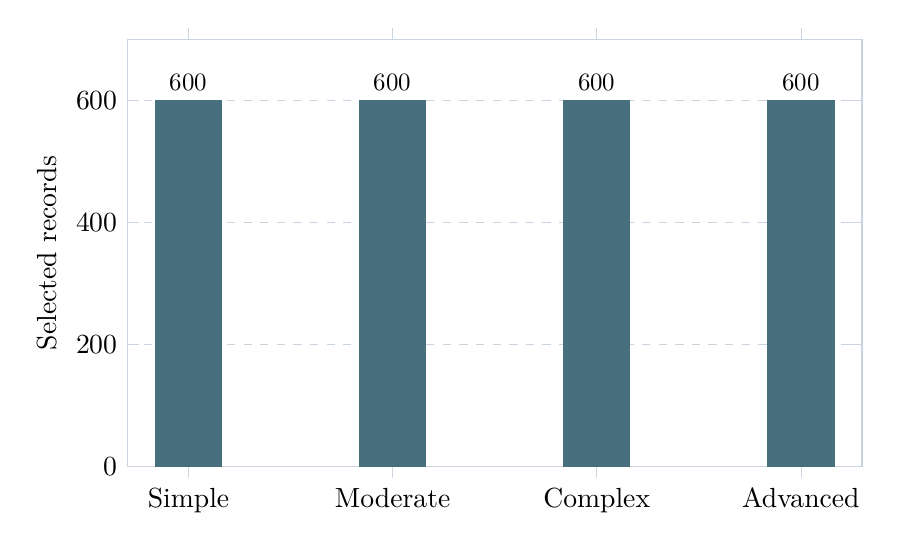
\begin{tikzpicture}
    \begin{axis}[
      ybar,
      width=0.9\textwidth,
      height=7cm,
      ymin=0,
      ymax=700,
      ylabel={Selected records},
      symbolic x coords={Simple,Moderate,Complex,Advanced},
      xtick=data,
      nodes near coords,
      nodes near coords align={vertical},
      bar width=24pt,
      axis line style={draw=aragline},
      tick style={draw=aragline},
      ymajorgrids=true,
      grid style={draw=aragline,dashed},
      every node near coord/.append style={font=\small}
    ]
      \addplot[fill=aragprimary,draw=aragprimary] coordinates {
        (Simple,600) (Moderate,600) (Complex,600) (Advanced,600)
      };
    \end{axis}
  \end{tikzpicture}
  \caption{Balanced four-class classifier dataset after deterministic preparation.}
  \label{fig:dataset-distribution}
\end{figure}


Records are split using source-document groups rather than independent random
rows. Questions that share a source group cannot appear in both training and
validation. With seed 42, the manifest contains \PreparedSourceGroups{} source
groups, \PreparedTrainRecords{} training records, and
\PreparedValidationRecords{} validation records. The validation class counts
are 120 simple, 119 moderate, 119 complex, and 123 advanced. The audit reports
no duplicate IDs, duplicate question groups, conflicting labels, or
train/validation source leakage.

\section{Classifier Training and Routing}

Two model families were trained and evaluated on the same source-grouped
validation split:

\begin{enumerate}
  \item DistilBERT sequence classification with four logits, softmax
  probabilities, confidence, top-two margin, and calibrated validation
  outputs; and
  \item T5-small sequence scoring over the four candidate labels, followed by
  probability normalization.
\end{enumerate}

The common interface preserves \Code{predict(query) -> label} and adds a scored
prediction containing probabilities, confidence, margin, deployment identity,
runtime, and latency. Comparison metrics include accuracy, macro F1,
per-label recall, advanced precision/recall/F1, expected calibration error,
latency, under-routing, over-routing, and route-cost regret.

Adaptive routing maps simple to L1, moderate to L2, complex to L3, and advanced
to L4. A low-confidence prediction may be escalated one route when confidence
is below 0.60 or top-two margin below 0.15. Saved configurations can change
these thresholds. Explicit L1--L4 mode does not use escalation, which is
necessary for controlled route experiments. A selected classifier failure
falls back to the process-default classifier and produces a prominent trace
warning.

\begin{figure}[H]
  \centering
  \resizebox{0.98\textwidth}{!}{%
  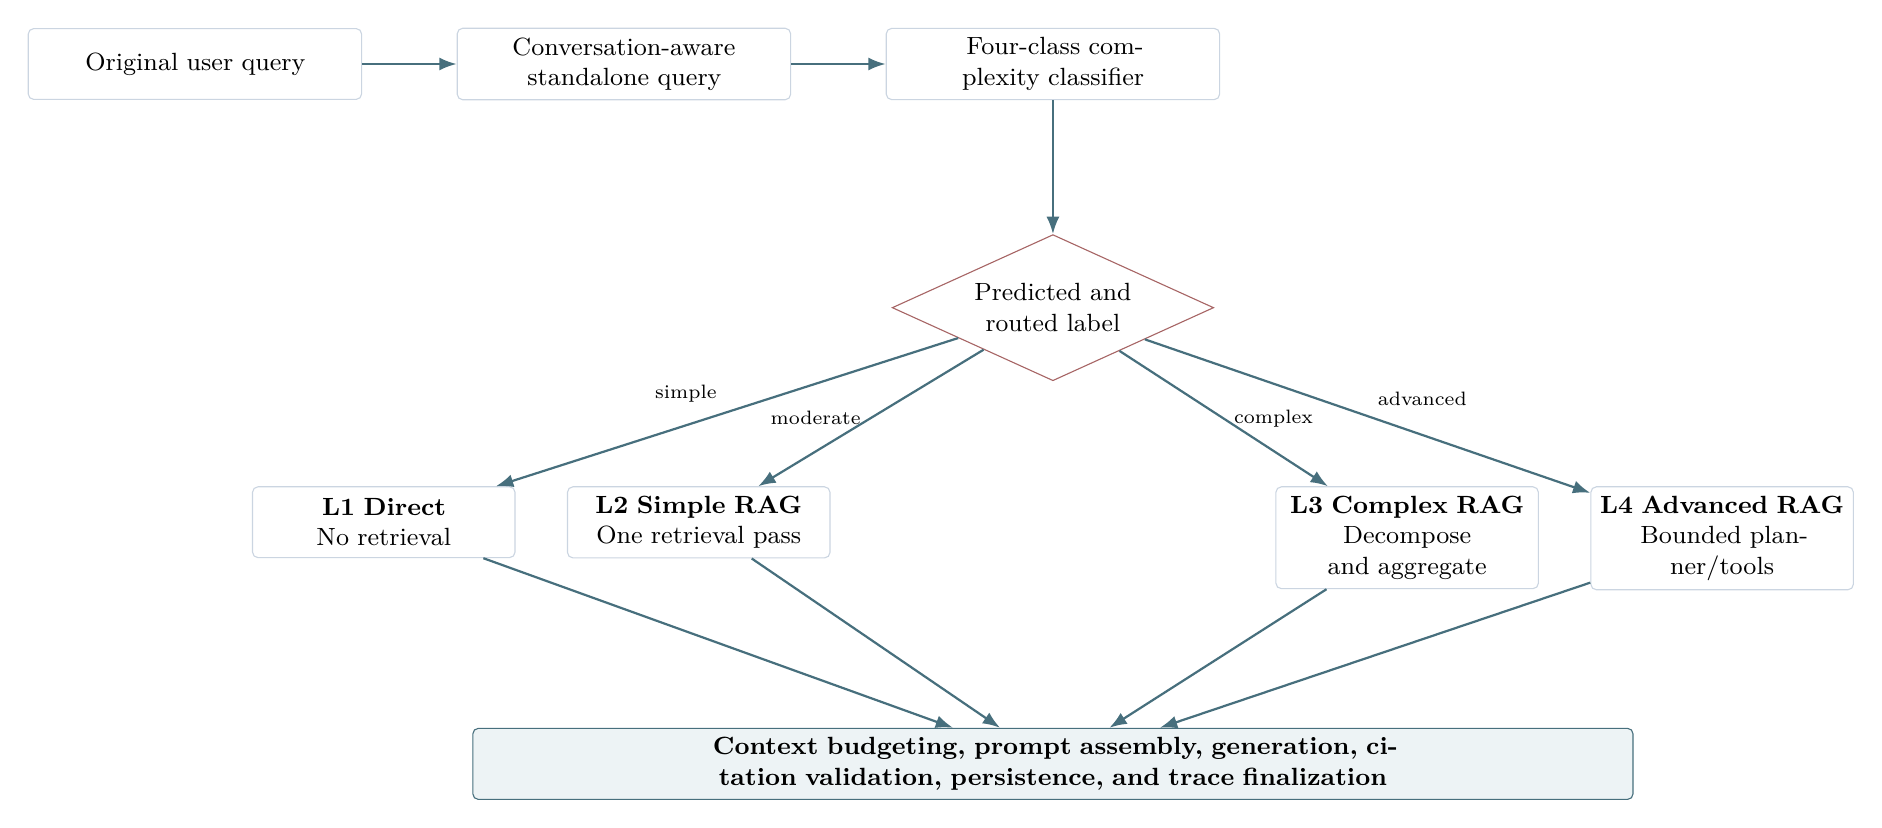
\begin{tikzpicture}[node distance=10mm and 12mm]
    \node[aragbox,text width=40mm] (query) {Original user query};
    \node[aragbox,text width=40mm,right=of query] (rewrite) {Conversation-aware standalone query};
    \node[aragbox,text width=40mm,right=of rewrite] (classifier) {Four-class complexity classifier};

    \node[aragdecision,below=17mm of classifier] (route) {Predicted and\\routed label};
    \node[aragbox,text width=31mm,below left=18mm and 58mm of route] (l1) {\textbf{L1 Direct}\\No retrieval};
    \node[aragbox,text width=31mm,below left=18mm and 18mm of route] (l2) {\textbf{L2 Simple RAG}\\One retrieval pass};
    \node[aragbox,text width=31mm,below right=18mm and 18mm of route] (l3) {\textbf{L3 Complex RAG}\\Decompose and aggregate};
    \node[aragbox,text width=31mm,below right=18mm and 58mm of route] (l4) {\textbf{L4 Advanced RAG}\\Bounded planner/tools};
    \node[araglayer,text width=145mm,below=17mm of route,yshift=-27mm] (generate) {Context budgeting, prompt assembly, generation, citation validation, persistence, and trace finalization};

    \draw[aragarrow] (query) -- (rewrite);
    \draw[aragarrow] (rewrite) -- (classifier);
    \draw[aragarrow] (classifier) -- (route);
    \draw[aragarrow] (route) -- node[above left,font=\scriptsize]{simple} (l1);
    \draw[aragarrow] (route) -- node[left,font=\scriptsize]{moderate} (l2);
    \draw[aragarrow] (route) -- node[right,font=\scriptsize]{complex} (l3);
    \draw[aragarrow] (route) -- node[above right,font=\scriptsize]{advanced} (l4);
    \draw[aragarrow] (l1) -- (generate);
    \draw[aragarrow] (l2) -- (generate);
    \draw[aragarrow] (l3) -- (generate);
    \draw[aragarrow] (l4) -- (generate);
  \end{tikzpicture}}
  \caption{Adaptive query routing from L1 to L4. L4 is an extension introduced by this project.}
  \label{fig:adaptive-routes}
\end{figure}


\section{Knowledge and Index Processing}

\subsection{Source Loading and Safety}

The source registry supports TXT, JSON, JSONL, Markdown, PDF, and DOCX uploads,
prepared WixQA corpus records, and public website URLs. Custom \texttt{aratxt},
\texttt{arajson}, and \texttt{aramd} extensions remain disabled until their
schemas are defined. Website loading rejects private-network destinations,
unsafe redirects, oversized responses, unsupported content types, and
timeouts, following SSRF-prevention principles \cite{owaspssrf2026}.

Each document receives source type, URI, MIME type, size, imported timestamp,
title, stable hash, and source-specific metadata. Deduplication occurs before
chunking. Prepared WixQA rows skip file parsing because their text and metadata
have already been normalized.

\subsection{Chunking}

Existing knowledge bases can use fixed-size, sliding-overlap, header-based,
recursive, semantic, parent-child, or structure-aware recursive chunking.
Legacy configurations retain character-based behavior. The WixQA MiniLM
profile uses the exact MiniLM BERT tokenizer and applies the settings in
\Cref{tab:wixqa-chunk-profile}.

\begin{table}[H]
  \centering
  \caption{WixQA MiniLM structure-aware chunking profile.}
  \label{tab:wixqa-chunk-profile}
  \begin{tabularx}{\textwidth}{p{0.34\textwidth}X}
    \toprule
    Parameter & Configured behavior\\
    \midrule
    Parent identity & WixQA article ID; chunks never cross articles.\\
    Target and soft body size & 180 and 210 WordPieces.\\
    Minimum and overlap & 60 and up to 30 WordPieces.\\
    Hard embedding input limit & 240 WordPieces including prefix and special tokens.\\
    Separator order & Heading, subheading, paragraph, list, sentence, token.\\
    Metadata prefix & Title and heading path, capped at 40 WordPieces.\\
    Structural rules & Preserve fitting numbered/bullet lists, merge small
    adjacent chunks, and overlap only inside the same section.\\
    \bottomrule
  \end{tabularx}
\end{table}

Stored chunk text remains clean. The title and section prefix is composed only
for embedding. Diagnostics store article ID, heading path, section ID, body,
prefix, embedding, and overlap token counts, profile ID, forced-split flag, and
below-minimum warning.

\subsection{Embedding and Atomic Indexes}

Knowledge bases select an embedding deployment and whether external processing
is permitted. Ingestion constructs the embedder from that KB configuration.
Remote embedding requires explicit egress permission and confirmation. The
same model, tokenizer limit, dimension, and active index version are applied to
query embeddings.

Indexing is asynchronous and durable. Chunks are embedded and persisted in
batches, a draft index version records the resolved configuration, and
activation occurs only after every batch succeeds. Failure or cancellation
leaves the previous index active. This prevents a query from observing a
partially built or mixed-model index.

\begin{figure}[H]
  \centering
  \resizebox{\textwidth}{!}{%
  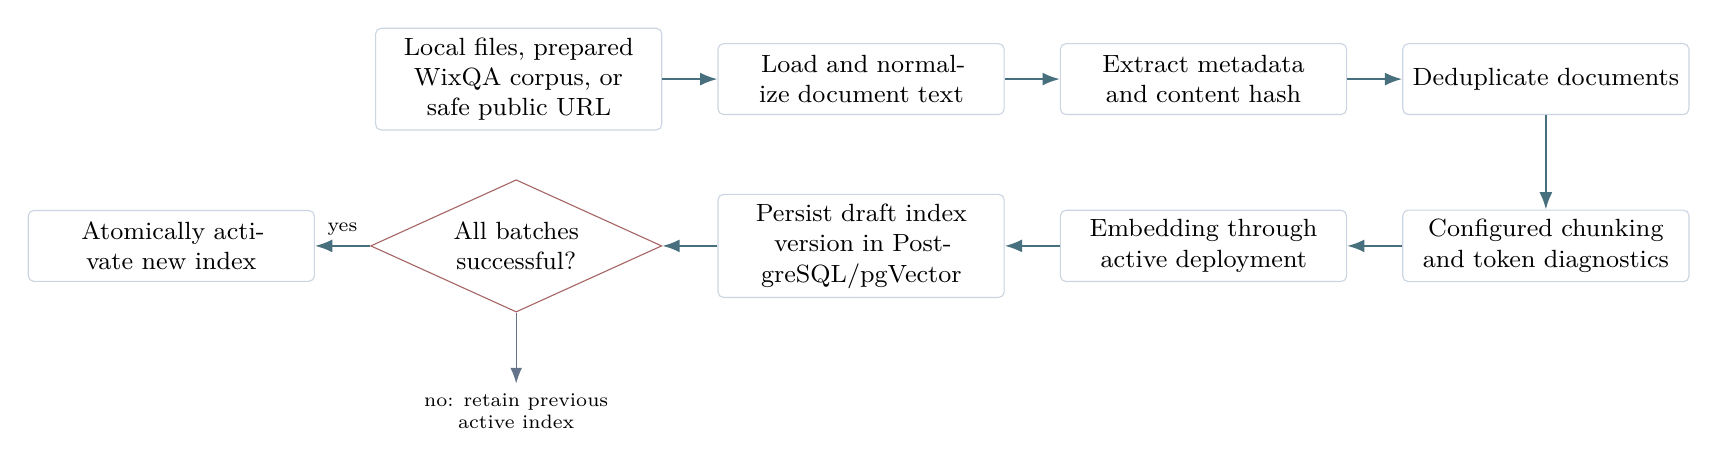
\begin{tikzpicture}[node distance=7mm]
    \node[aragbox] (source) {Local files, prepared WixQA corpus, or safe public URL};
    \node[aragbox,right=of source] (load) {Load and normalize document text};
    \node[aragbox,right=of load] (meta) {Extract metadata and content hash};
    \node[aragbox,right=of meta] (dedup) {Deduplicate documents};
    \node[aragbox,below=12mm of dedup] (chunk) {Configured chunking and token diagnostics};
    \node[aragbox,left=of chunk] (embed) {Embedding through active deployment};
    \node[aragbox,left=of embed] (draft) {Persist draft index version in PostgreSQL/pgVector};
    \node[aragdecision,left=of draft] (valid) {All batches\\successful?};
    \node[aragbox,left=of valid] (activate) {Atomically activate new index};

    \draw[aragarrow] (source) -- (load);
    \draw[aragarrow] (load) -- (meta);
    \draw[aragarrow] (meta) -- (dedup);
    \draw[aragarrow] (dedup) -- (chunk);
    \draw[aragarrow] (chunk) -- (embed);
    \draw[aragarrow] (embed) -- (draft);
    \draw[aragarrow] (draft) -- (valid);
    \draw[aragarrow] (valid) -- node[above,font=\scriptsize]{yes} (activate);
    \draw[aragsoftarrow] (valid.south) -- ++(0,-9mm) node[below,font=\scriptsize,align=center]{no: retain previous\\active index};
  \end{tikzpicture}}
  \caption{Versioned knowledge ingestion and index activation workflow.}
  \label{fig:knowledge-pipeline}
\end{figure}


\section{Query-Time Adaptive RAG}

\subsection{Conversation Context and Reformulation}

When enabled, the service loads only completed user--assistant exchanges that
precede the current request. Failed, cancelled, pending, and streaming messages
are excluded. The number of exchanges and character budget are configurable,
subject to server ceilings of six exchanges and 10,000 characters.
Evaluation disables conversation context because each benchmark case is an
independent QA observation.

Referential follow-ups are converted into a standalone query. Deterministic
rewriting is always available. A selected planner can perform the rewrite
through the Model Gateway; invalid output, provider failure, or blocked egress
falls back without failing the answer. The original query is retained for the
answer, while classification, retrieval, reranking, and decomposition use the
standalone query.

\subsection{Retrieval Routes}

L1 calls the generator without knowledge retrieval. L2 performs one configured
retrieval pass. BM25 uses a complete active-index lexical cache; dense search
uses pgVector; hybrid search normalizes and weights both result sets. A
document filter restricts all retrieval to selected document IDs.

L3 creates two to four subqueries, retaining the standalone query as the global
subquery. Each query is retrieved independently. Repeated chunks are
deduplicated by stable identity, then ranked using retrieval score, original
rank, and subquery coverage. Planner decomposition must return a validated JSON
list; otherwise deterministic decomposition is used.

L4 exposes only available, authorized tools: KB hybrid search, chunk/document
inspection, evidence reranking, SSRF-safe public URL retrieval when enabled,
and final-answer completion. The defaults are five planning iterations, eight
tool calls, and 90 seconds. Planner errors are structured observations that may
be recovered. A missing or repeatedly invalid planner falls back to L3.

\subsection{Prompting, Generation, and Citations}

Prompt construction combines system prompt, predefined instructions, response
structure, tone, humor level, bounded conversation history, original question,
standalone query, and labelled evidence. Retrieved contexts receive stable
labels such as \texttt{[S1]}. History and retrieved documents are explicitly
treated as untrusted context rather than system instructions.

The selected generator executes through the Model Gateway. Local extractive
generation provides a deterministic baseline; FLAN-T5 provides optional local
generation; remote or self-hosted models use LiteLLM. A fallback deployment is
permitted only for retryable failure and, during streaming, only before the
first text delta. Citation validation detects missing and unknown labels.
Validation is advisory: it returns a warning rather than triggering a second
paid generation call.

\section{Model Governance Method}

The AI Models catalog separates reusable provider connections from
deployments. Connections contain access path, API base, encrypted credentials,
locality, and health. Deployments contain provider-native model ID,
capabilities, parameters, limits, pricing, budget, health, and enabled status.
Only tested and enabled deployments appear in runtime selectors.

\begin{figure}[H]
  \centering
  \resizebox{\textwidth}{!}{%
  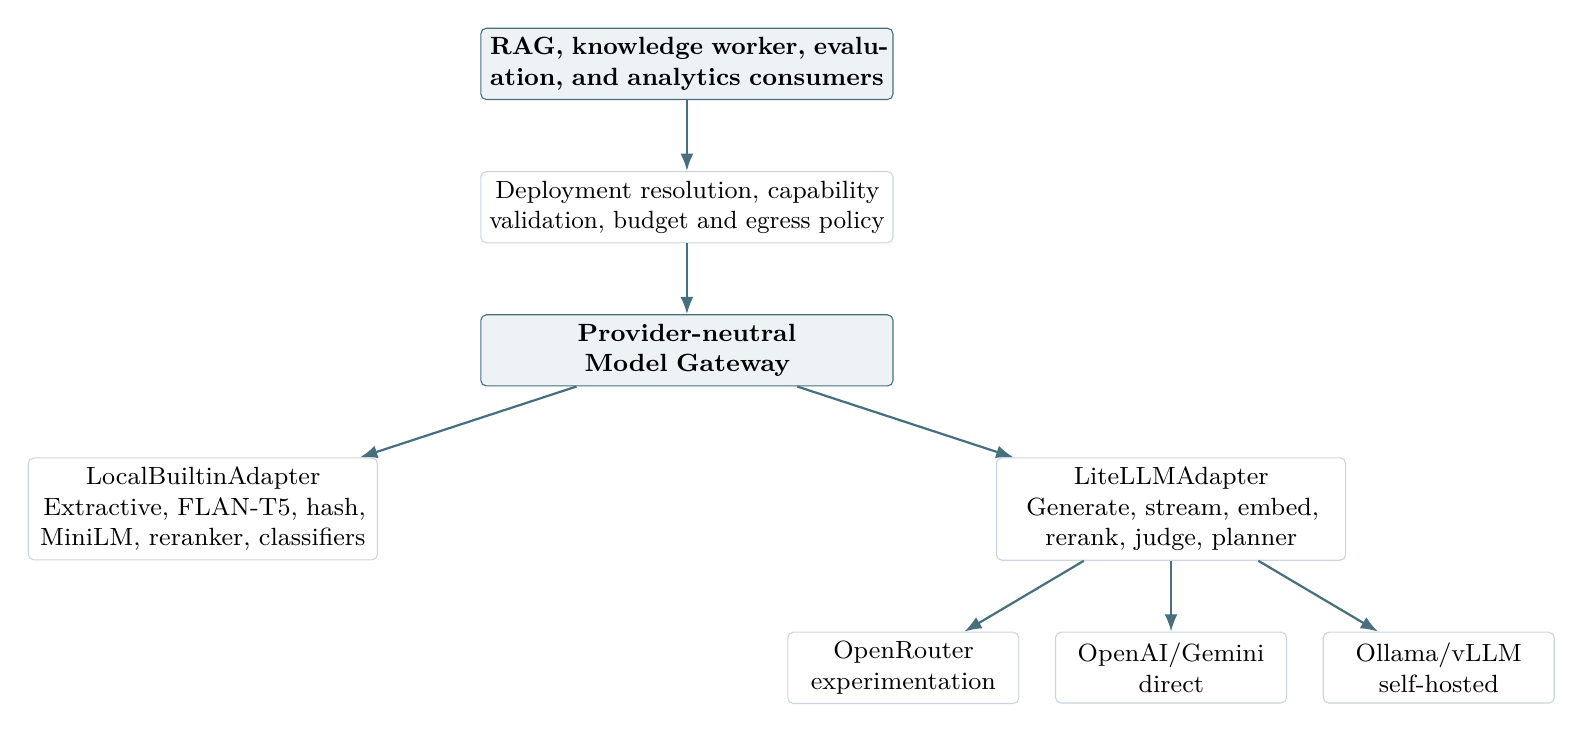
\begin{tikzpicture}[node distance=9mm and 13mm]
    \node[araglayer,text width=50mm] (consumer) {RAG, knowledge worker, evaluation, and analytics consumers};
    \node[aragbox,text width=50mm,below=of consumer] (policy) {Deployment resolution, capability validation, budget and egress policy};
    \node[araglayer,text width=50mm,below=of policy] (gateway) {Provider-neutral Model Gateway};
    \node[aragbox,text width=42mm,below left=of gateway] (builtin) {LocalBuiltinAdapter\\Extractive, FLAN-T5, hash, MiniLM, reranker, classifiers};
    \node[aragbox,text width=42mm,below right=of gateway] (lite) {LiteLLMAdapter\\Generate, stream, embed, rerank, judge, planner};
    \node[aragbox,text width=27mm,below=of lite,xshift=-34mm] (exp) {OpenRouter\\experimentation};
    \node[aragbox,text width=27mm,below=of lite] (direct) {OpenAI/Gemini\\direct};
    \node[aragbox,text width=27mm,below=of lite,xshift=34mm] (self) {Ollama/vLLM\\self-hosted};

    \draw[aragarrow] (consumer) -- (policy);
    \draw[aragarrow] (policy) -- (gateway);
    \draw[aragarrow] (gateway) -- (builtin);
    \draw[aragarrow] (gateway) -- (lite);
    \draw[aragarrow] (lite) -- (exp);
    \draw[aragarrow] (lite) -- (direct);
    \draw[aragarrow] (lite) -- (self);
  \end{tikzpicture}}
  \caption{Unified AI Model Gateway and runtime access paths.}
  \label{fig:model-gateway}
\end{figure}


Credentials entered through the UI are encrypted using a versioned AES-GCM
envelope. API responses expose only credential readiness, never the value.
Each model attempt records purpose, deployment, connection, requested and
resolved model, latency, tokens, estimated cost, status, fallback index, and
related conversation, KB, or evaluation identifiers. Embeddings never fall
back to a different model because that would violate vector compatibility.

\section{Evaluation Design}

An experiment selects one or more saved RAG configurations, one or more WixQA
subsets, a knowledge base, a judge deployment, a case limit, and deterministic
sampling seed. Each configuration--dataset cell runs independently. There is
no hidden static-L2 baseline; Adaptive and L2 are compared by selecting two
saved configurations.

\begin{table}[H]
  \centering
  \caption{Evaluation dimensions and representative metrics.}
  \label{tab:evaluation-metrics}
  \begin{tabularx}{\textwidth}{p{0.24\textwidth}X}
    \toprule
    Dimension & Metrics\\
    \midrule
    Routing & Accuracy, macro F1, confusion matrix, per-label recall,
    under-routing, over-routing, route distribution, route-cost regret.\\
    Retrieval & Hit@\textit{k}, MRR, precision@\textit{k}, recall@\textit{k},
    NDCG@\textit{k}, retrieval coverage, context relevancy, context recall.\\
    Generation & Token F1, BLEU, ROUGE-1, ROUGE-2, answer overlap,
    factuality, context adherence, answer relevancy, grading note.\\
    Operations & End-to-end and stage latency, tokens, estimated cost, model
    calls, retrieved contexts, failures, cancellations, and fallback use.\\
    Human feedback & Per-answer-version thumbs up/down and optional comment,
    linked to configuration, KB, user, and trace.\\
    \bottomrule
  \end{tabularx}
\end{table}

Judge calls use structured output and one malformed-JSON repair attempt. Runs
remain failed rather than silently complete when required metrics are absent.
RAGXplain diagnosis is a separate bounded job over selected cases. This avoids
unexpected judge costs and allows normal evaluation results to remain valid if
diagnosis fails.

\begin{figure}[H]
  \centering
  \resizebox{\textwidth}{!}{%
  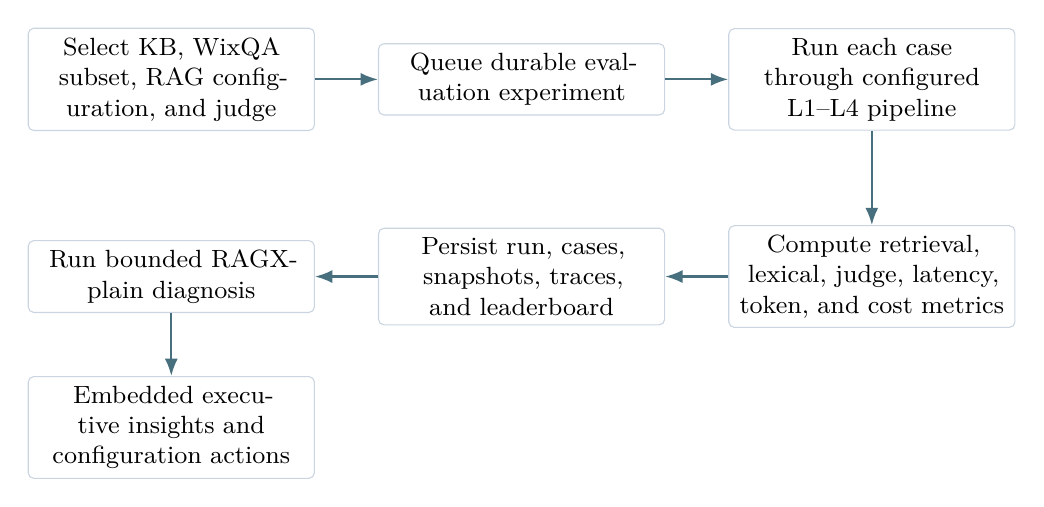
\begin{tikzpicture}[node distance=8mm]
    \node[aragbox] (select) {Select KB, WixQA subset, RAG configuration, and judge};
    \node[aragbox,right=of select] (queue) {Queue durable evaluation experiment};
    \node[aragbox,right=of queue] (execute) {Run each case through configured L1--L4 pipeline};
    \node[aragbox,below=12mm of execute] (metrics) {Compute retrieval, lexical, judge, latency, token, and cost metrics};
    \node[aragbox,left=of metrics] (persist) {Persist run, cases, snapshots, traces, and leaderboard};
    \node[aragbox,left=of persist] (diagnose) {Run bounded RAGXplain diagnosis};
    \node[aragbox,below=of diagnose] (viewer) {Embedded executive insights and configuration actions};

    \draw[aragarrow] (select) -- (queue);
    \draw[aragarrow] (queue) -- (execute);
    \draw[aragarrow] (execute) -- (metrics);
    \draw[aragarrow] (metrics) -- (persist);
    \draw[aragarrow] (persist) -- (diagnose);
    \draw[aragarrow] (diagnose) -- (viewer);
  \end{tikzpicture}}
  \caption{Configuration-based WixQA evaluation and RAGXplain diagnosis workflow.}
  \label{fig:evaluation-workflow}
\end{figure}


\section{Validity, Reproducibility, and Ethics}

Internal validity is supported by immutable configuration snapshots,
deterministic sampling, grouped splits, artifact hashes, route traces, and
recorded model identities. Construct validity remains limited because lexical
overlap and LLM judges approximate answer quality. External validity is limited
to Wix business support content and the configurations actually tested.
Conclusion validity remains limited by the 20-case compatible sample reported
in \Cref{chap:implementation-results}; larger controlled samples are required
for statistical claims.

The repository records the Git commit, Python version, model deployment, KB
index, prompts, and evaluation settings. Full traces improve reproducibility
but may contain prompts and retrieved enterprise content. They are retained for
a bounded period, compressed, size-limited, and sanitized to exclude secrets,
authorization headers, encrypted credentials, and raw numerical vectors.
Remote processing is blocked unless enabled for the KB, providing an explicit
data-egress decision.

\chapter{Implementation and Results}
\label{chap:implementation-results}

\section{System Overview}

\SystemName{} is implemented as a Python 3.11 package, FastAPI application,
React frontend, PostgreSQL/pgVector database, and background worker. The
architecture in \Cref{fig:overall-architecture} separates application,
orchestration, knowledge processing, model, evaluation, governance, agent,
prompt-engineering, and storage responsibilities.

\begin{landscape}
  \begin{figure}[p]
    \centering
    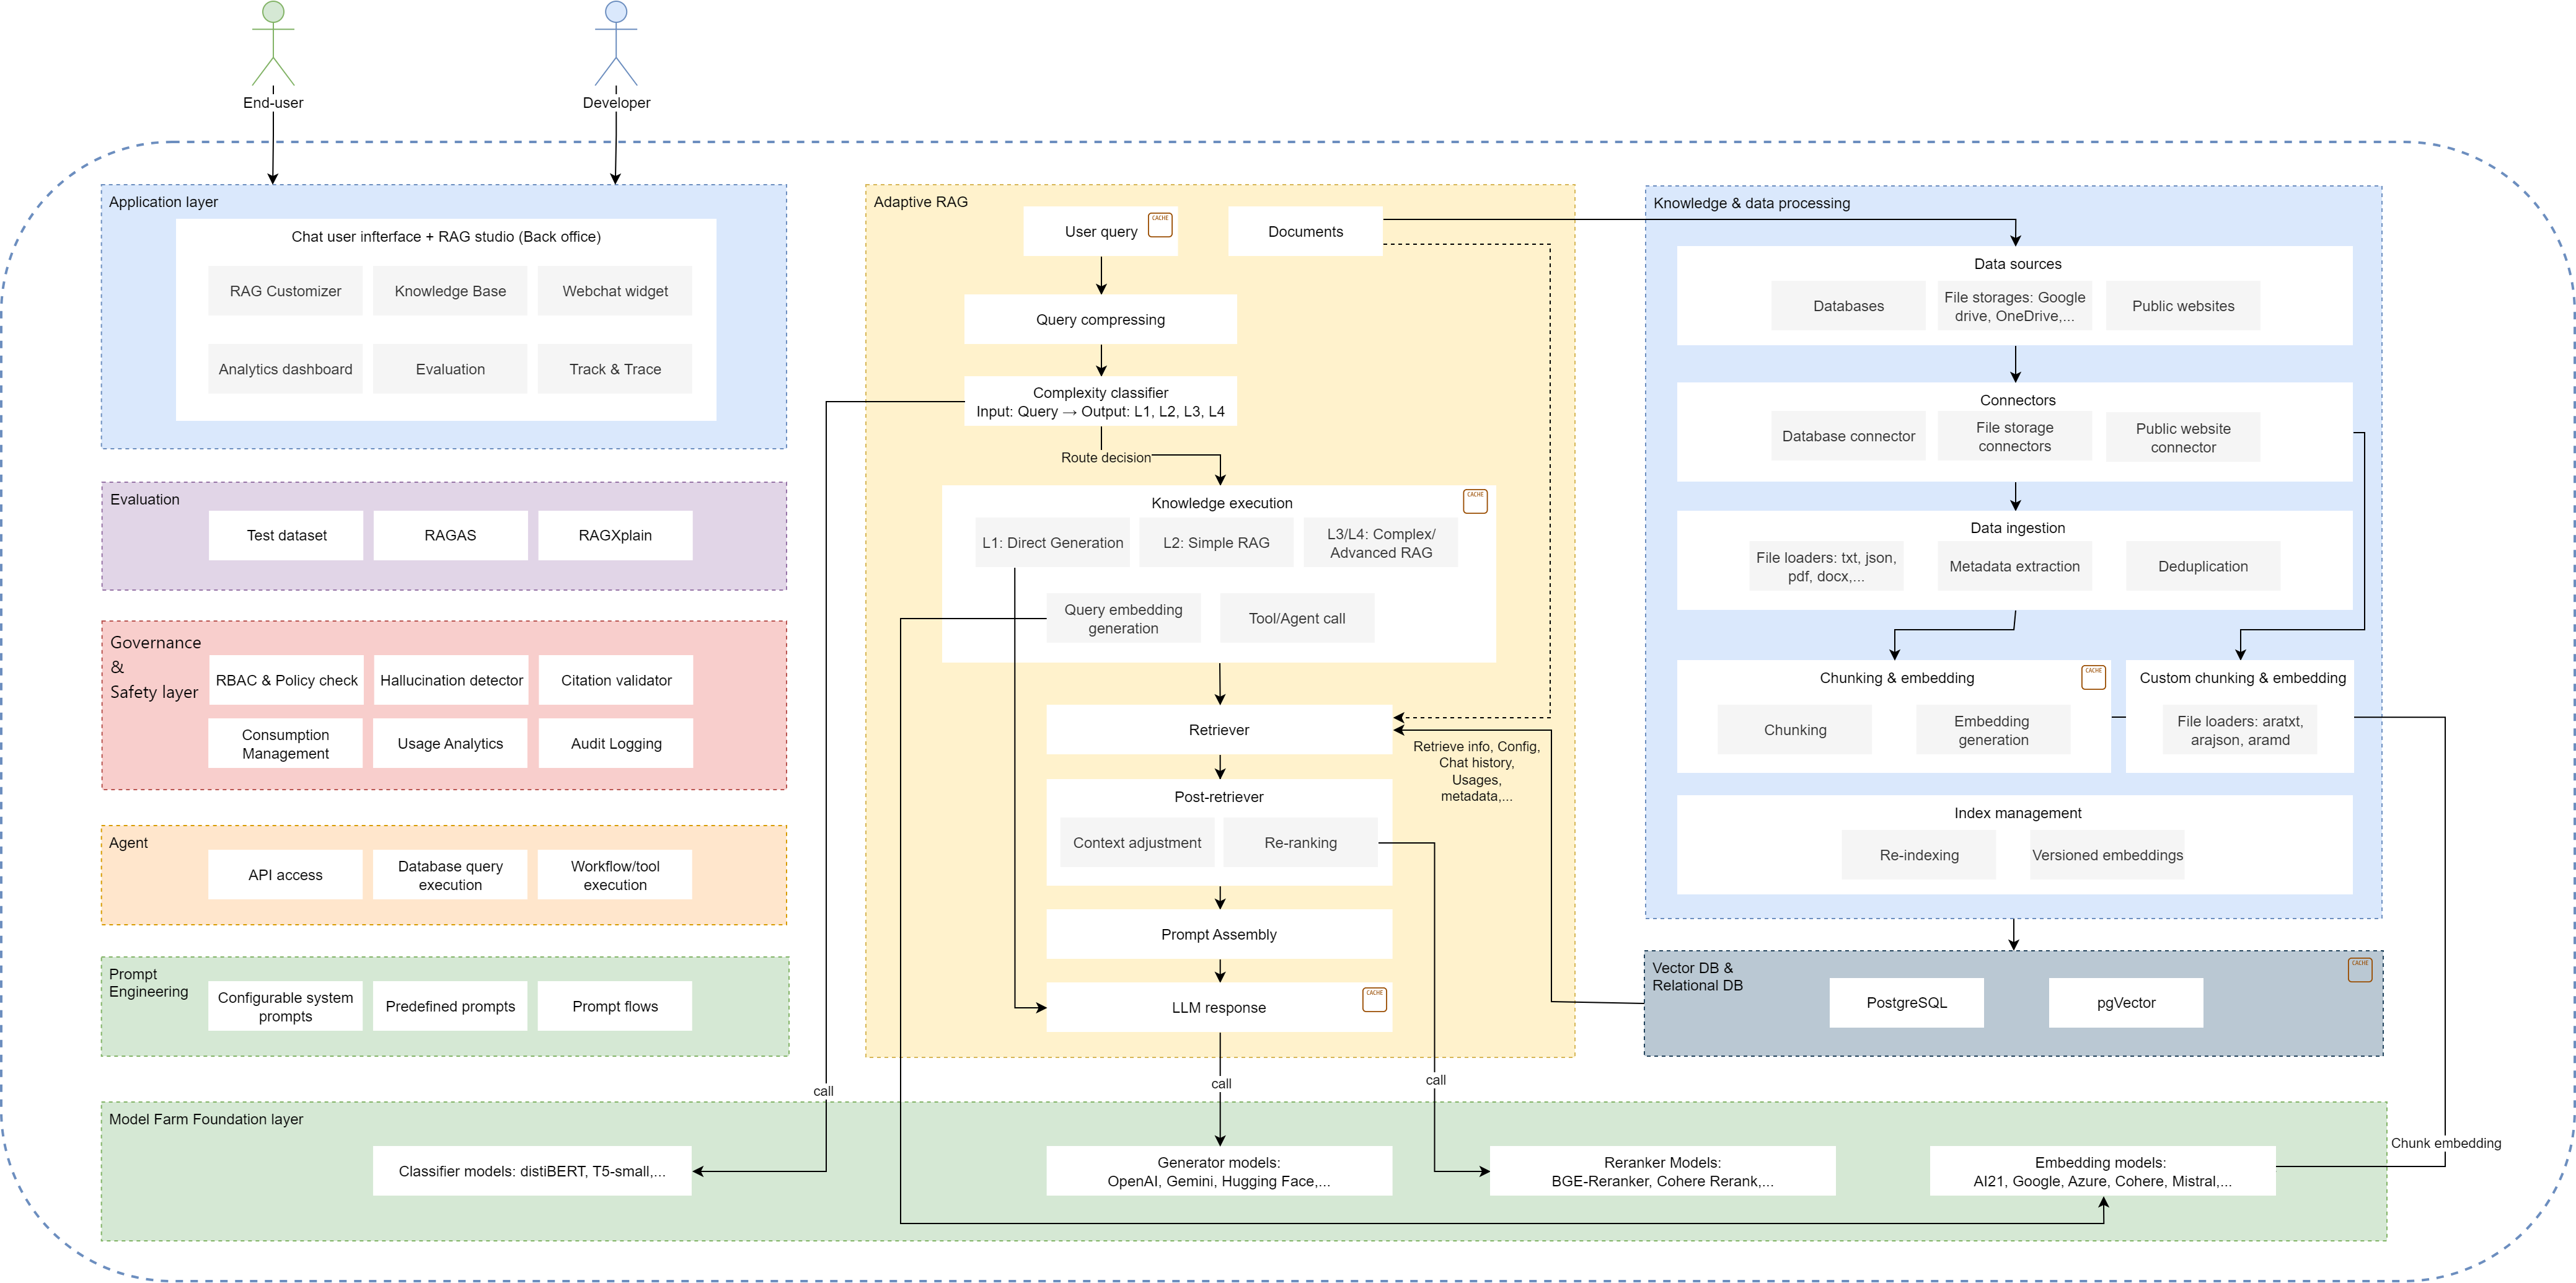
\includegraphics[width=0.98\linewidth,height=0.82\textheight,keepaspectratio]{figures/architecture_landscape.png}
    \caption{Implemented layered architecture of the \SystemName{} system.}
    \label{fig:overall-architecture}
  \end{figure}
\end{landscape}

The separation is behavioral rather than cosmetic. Knowledge ingestion can be
tested without running the React UI. The answer service can use a JSON
repository for bounded tests or PostgreSQL for the full system. Model providers
are selected by deployment ID rather than imported directly into RAG logic.
Evaluation calls the same answer orchestration used by chat, avoiding a
parallel benchmark-only implementation.

\section{Application and API Layer}

The React studio provides Main, Knowledge Bases, AI Models, Evaluation, and
Analytics screens under an authenticated top navigation. FastAPI validates
requests, resolves the current user and role, enforces resource policies, and
returns synchronous JSON or SSE. JWT-backed local users have \texttt{admin} or
\texttt{user} roles. AI Models and organization-wide analytics are restricted
to administrators, while authenticated users can chat and submit feedback.

The Main screen uses three resizable panels:

\begin{enumerate}
  \item an Explorer with New Chat, search, pinned Library, and recent
  conversations;
  \item the chat panel with persistent messages, document filtering, streaming,
  citations, sources, traces, feedback, answer versions, Stop, Retry, and
  Regenerate; and
  \item the RAG Customizer with Knowledge Base status, General settings,
  Adaptive RAG controls, and generator/prompt controls.
\end{enumerate}

Panel widths and collapsed state persist in browser storage. Conversation
history, configuration snapshots, contexts, trace IDs, message states, and
answer versions persist on the server. This means restoring a chat also
restores source links, citation warnings, follow-up-rewrite markers, and trace
navigation.

\ReportAsset{ui-main.png}{Main screen with Explorer, streaming chat, and RAG Customizer.}{fig:ui-main}

\section{Knowledge Base Implementation}

The Knowledge Bases screen manages a one-to-many relationship between a
knowledge base and its documents. A shared Add/Modify dialog captures name,
description, source, chunking profile, embedding deployment, and external
processing policy. Documents are browsed with server-side search and
pagination. Expanding a document lazily loads its chunks and displays metadata,
embedding identity, and processing trace.

Local upload and prepared WixQA import are operational. Public websites use the
safety policy described in \Cref{chap:methodology}. Google Drive, OneDrive, and
database sources are visible extension points but unavailable. Prepared WixQA
import can select a deterministic document count rather than requiring the
entire corpus. Evaluation compatibility records the selected source IDs so a
benchmark can sample only cases grounded in those documents.

Ingestion, re-indexing, and corpus import are durable jobs. The worker claims
leased jobs with PostgreSQL locking, updates bounded progress stages, and
checks cancellation between batches. Uploads are staged by content hash.
Unchanged chunks can reuse embeddings. A failed draft does not replace the
active index.

\ReportAsset{ui-knowledge-bases.png}{Knowledge Base management, paginated documents, and processing details.}{fig:ui-knowledge}

\section{AI Models and Model Gateway}

AI Models presents deployments as smaller grouped cards under Experimentation,
Production Direct, and Local. A single consistent-width wizard selects a
provider or local model, captures connection details, tests the endpoint, saves
it, then creates and enables a deployment. Editing uses the same flow.

Connections and deployments are separate database entities. For example, one
OpenRouter connection may support several deployments with different
provider-native model IDs and capabilities. Stored model IDs are normalized at
runtime:

\begin{table}[H]
  \centering
  \caption{Representative runtime model-ID mapping.}
  \label{tab:model-id-mapping}
  \begin{tabularx}{\textwidth}{p{0.2\textwidth}p{0.34\textwidth}X}
    \toprule
    Connection & Stored model ID & LiteLLM runtime ID\\
    \midrule
    OpenRouter & \texttt{google/gemma-\ldots} & \texttt{openrouter/google/gemma-\ldots}\\
    OpenAI direct & \texttt{gpt-4.1-mini} & \texttt{gpt-4.1-mini}\\
    Gemini direct & \texttt{gemini-2.5-flash} & \texttt{gemini/gemini-2.5-flash}\\
    Ollama & \texttt{llama3.1} & \texttt{ollama\_chat/llama3.1}\\
    vLLM & server model name & \texttt{hosted\_vllm/<model>}\\
    \bottomrule
  \end{tabularx}
\end{table}

The gateway exposes generation, streaming, embedding, reranking,
classification, planning, judging, and health testing. Local built-ins include
extractive generation, FLAN-T5, hash-384 embedding, MiniLM-384, lexical
reranking, and classifier deployments. Remote calls use one LiteLLM boundary.
Credential values are encrypted before storage and redacted from responses,
errors, usage, and traces.

\ReportAsset{ui-ai-models.png}{AI Models catalog and connection/deployment workflow.}{fig:ui-models}

\section{Adaptive RAG Runtime}

The async answer service prepares a request through policy, conversation
context, reformulation, classification, route selection, retrieval, reranking,
context budgeting, prompt assembly, generation, citation validation,
persistence, and telemetry. Synchronous and streaming endpoints reuse these
stages.

\subsection{Runtime-Truthful Configuration}

Every Main-screen Adaptive RAG control is connected to execution:

\begin{itemize}
  \item the selected classifier controls Adaptive routing, with explicit
  configured/actual/fallback metadata;
  \item the selected planner can rewrite follow-ups, decompose L3 queries, and
  drive bounded L4 actions;
  \item the query embedding is inherited from the active KB index and cannot be
  overridden by a stale chat configuration;
  \item BM25 avoids an embedding call; dense and hybrid retrieval use the
  active index deployment;
  \item reranking executes only when enabled and a compatible deployment is
  selected;
  \item citation settings modify the prompt and validation; and
  \item generator, fallbacks, prompts, style, history, and agent limits are
  preserved in configuration and conversation snapshots.
\end{itemize}

This design addresses a common prototype defect where controls are stored as
metadata but do not affect runtime. Trace summaries distinguish what was
configured from what actually executed.

\subsection{Streaming and Answer Lifecycle}

The streaming endpoint sends \texttt{started}, \texttt{trace},
\texttt{sources}, and \texttt{delta} progress events. It terminates with
\texttt{model\_completed}, \texttt{completed}, \texttt{cancelled}, or
\texttt{error}. LiteLLM
providers stream deltas directly. FLAN-T5 uses a background generation thread
and iterator. The deterministic extractive generator emits bounded chunks.

\begin{figure}[H]
  \centering
  \resizebox{\textwidth}{!}{%
  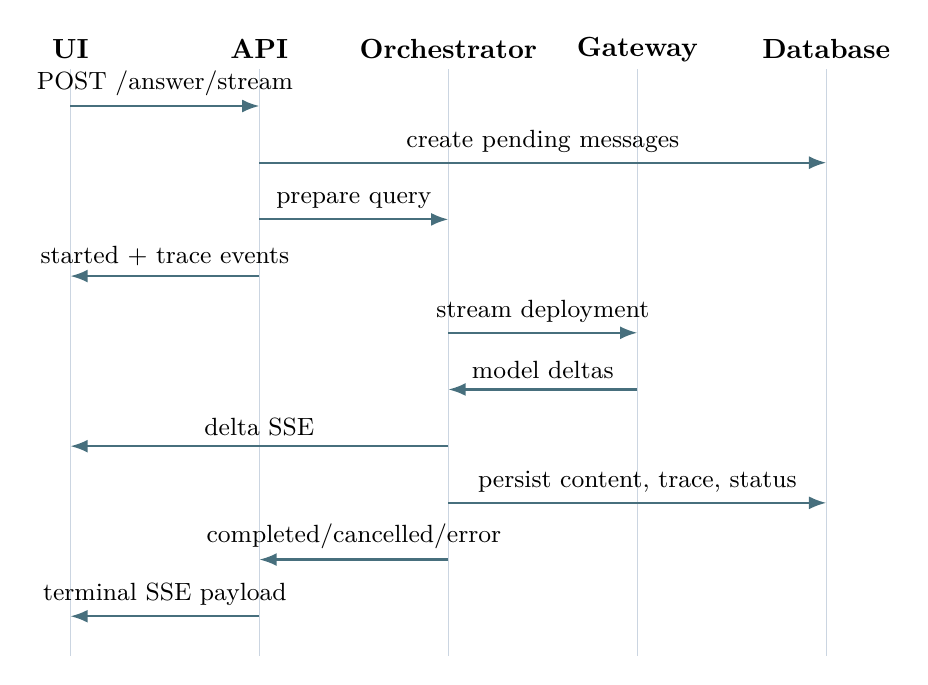
\begin{tikzpicture}[x=2.4cm,y=0.72cm,font=\small]
    \foreach \name/\x in {UI/0,API/1,Orchestrator/2,Gateway/3,Database/4} {
      \node[font=\bfseries] at (\x,0) {\name};
      \draw[aragline] (\x,-0.35) -- (\x,-10.7);
    }
    \draw[aragarrow] (0,-1) -- node[above]{POST /answer/stream} (1,-1);
    \draw[aragarrow] (1,-2) -- node[above]{create pending messages} (4,-2);
    \draw[aragarrow] (1,-3) -- node[above]{prepare query} (2,-3);
    \draw[aragarrow] (1,-4) -- node[above]{started + trace events} (0,-4);
    \draw[aragarrow] (2,-5) -- node[above]{stream deployment} (3,-5);
    \draw[aragarrow] (3,-6) -- node[above]{model deltas} (2,-6);
    \draw[aragarrow] (2,-7) -- node[above]{delta SSE} (0,-7);
    \draw[aragarrow] (2,-8) -- node[above]{persist content, trace, status} (4,-8);
    \draw[aragarrow] (2,-9) -- node[above]{completed/cancelled/error} (1,-9);
    \draw[aragarrow] (1,-10) -- node[above]{terminal SSE payload} (0,-10);
  \end{tikzpicture}}
  \caption{True provider streaming and durable message-state sequence.}
  \label{fig:streaming-sequence}
\end{figure}


Messages and answer versions use pending, streaming, completed, failed, and
cancelled states. Explicit Stop and client disconnect converge on one
cancellation path. A successful regeneration becomes the canonical assistant
message while preserving previous versions. A failed retry retains partial
content and leaves the prior successful canonical answer unchanged.

\section{Retrieval, Sources, and Grounded Citations}

The retriever supports complete active-index BM25, pgVector dense similarity,
and normalized hybrid ranking. Lexical indexes are cached by KB and active
index version with bounded eviction. A document filter indexes or searches only
selected documents. L3 diagnostics retain subquery, retrieval step, original
rank, aggregated rank, and coverage.

Retrieved chunks receive source labels. Markdown rendering converts valid
labels such as \texttt{[S1]} into accessible buttons, except inside code or
existing links. Clicking a citation opens the Source dialog at the stable chunk
identity. Unknown labels remain visually invalid and appear in the citation
validation trace.

The Source dialog has a searchable selectable list and one focused preview.
It shows rank, score, retrieval mode, document, chunk index, embedding model,
and L3/L4 metadata. The Trace dialog can navigate from a retrieval candidate
to the same source preview.

\section{Observability}

Every answer can produce a versioned, strict UTF-8 trace. PostgreSQL stores
searchable metadata while a gzip artifact stores hierarchical spans. Each span
has stable IDs, parent, sequence, category, status, timestamps, duration,
sanitized inputs/outputs, metrics, model usage IDs, warnings, and errors.
Partial traces are persisted at completed-span boundaries, preserving evidence
for failure and cancellation.

\begin{figure}[H]
  \centering
  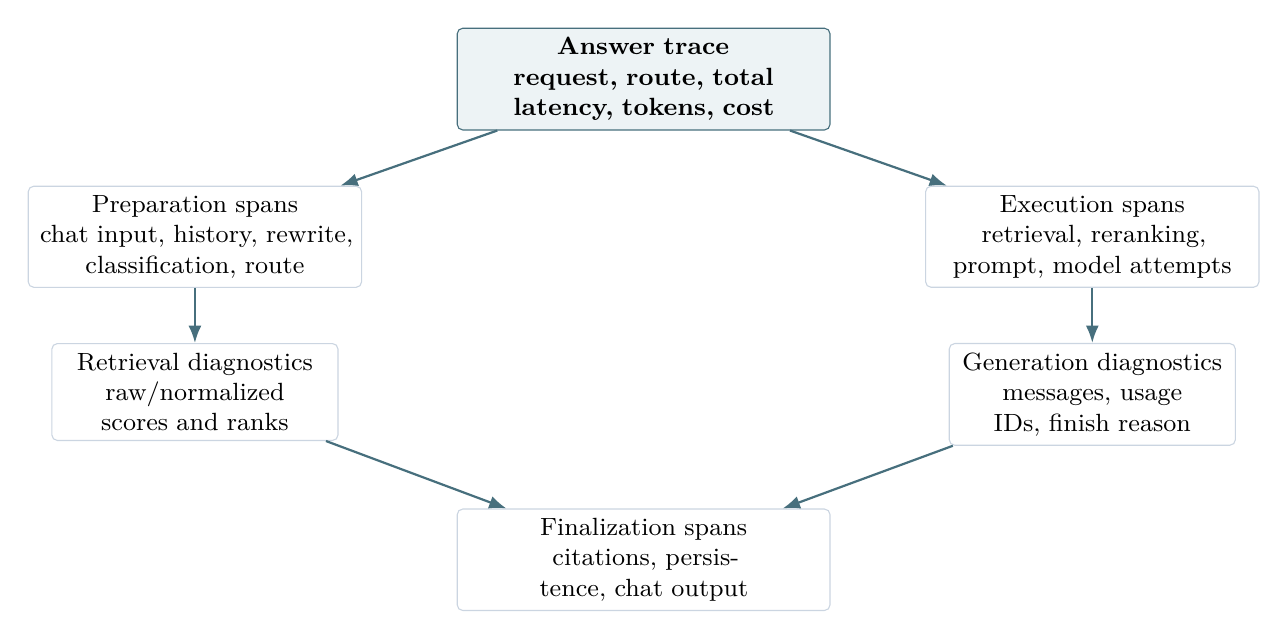
\begin{tikzpicture}[node distance=7mm and 12mm]
    \node[araglayer,text width=45mm] (trace) {Answer trace\\request, route, total latency, tokens, cost};
    \node[aragbox,text width=40mm,below left=of trace] (prepare) {Preparation spans\\chat input, history, rewrite, classification, route};
    \node[aragbox,text width=40mm,below right=of trace] (execution) {Execution spans\\retrieval, reranking, prompt, model attempts};
    \node[aragbox,text width=34mm,below=of prepare] (retrieval) {Retrieval diagnostics\\raw/normalized scores and ranks};
    \node[aragbox,text width=34mm,below=of execution] (generation) {Generation diagnostics\\messages, usage IDs, finish reason};
    \node[aragbox,text width=45mm,below=16mm of trace,yshift=-32mm] (final) {Finalization spans\\citations, persistence, chat output};

    \draw[aragarrow] (trace) -- (prepare);
    \draw[aragarrow] (trace) -- (execution);
    \draw[aragarrow] (prepare) -- (retrieval);
    \draw[aragarrow] (execution) -- (generation);
    \draw[aragarrow] (retrieval) -- (final);
    \draw[aragarrow] (generation) -- (final);
  \end{tikzpicture}
  \caption{Hierarchical full-fidelity observability trace model.}
  \label{fig:trace-hierarchy}
\end{figure}


The trace UI shows total latency, tokens, cost, route, models, warnings, a
waterfall, and hierarchical stages. The orchestration root appears in the
waterfall but is not numbered as a pipeline step. Step details provide Inputs,
Outputs, Metrics, Model Usage, and Raw JSON tabs. Summary and waterfall regions
can collapse to prioritize the selected detail.

Artifacts exclude API keys, authorization headers, encrypted credentials, and
raw embedding vectors. The default maximum compressed artifact size is 10 MB
and retention is 30 days. Truncated sections remain valid JSON and record the
reason.

\ReportAsset{ui-trace.png}{Full-fidelity Trace report with waterfall and selected-span details.}{fig:ui-trace}

\section{Evaluation and RAGXplain}

The Evaluation screen creates durable configuration-based experiment matrices.
Each selected saved configuration runs exactly once per selected dataset cell.
The UI shows progress, metric cards, route distribution, leaderboard, and
case-level Trace actions. WixQA eligibility detects mismatched corpus subsets
rather than comparing queries against unrelated KB documents.

The RAGXplain adapter exports question, candidate answer, contexts, and ground
truth, then uses the selected Model Farm judge for six semantic metrics. It
validates that semantic score columns and insight summaries exist before
reporting completion. The embedded viewer automatically loads
\texttt{overall\_insights.json}; no manual upload panel is shown in the normal
flow.

\ReportAsset{ui-evaluation.png}{Configuration-based WixQA experiment and selected-run metrics.}{fig:ui-evaluation}
\ReportAsset{ragxplain-insights.png}{Embedded RAGXplain executive summary and action protocols.}{fig:ui-ragxplain}

\section{Analytics and Feedback}

Analytics is an administrator-only PostgreSQL dashboard. Token Statistics
provides date and dimension filters, totals, daily token/cost trends,
breakdowns by model, KB, configuration, and purpose, and paginated usage
events. Detailed Statistics and Feedbacks reports active conversations,
messages, authenticated active users, and ratings. Tables support server
pagination, filters, column resizing, and horizontal scrolling.

Feedback is attached to one assistant answer version per user. The server
derives the KB, configuration, question, answer, and trace rather than trusting
client snapshots. A rating change updates the same record. The feedback table
links to the exact trace when a durable trace ID is available.

\ReportAsset{ui-analytics.png}{Usage, cost, engagement, and structured feedback analytics.}{fig:ui-analytics}

\section{Deployment and Persistence}

Docker Compose defines PostgreSQL/pgVector, migration, API, and worker services.
Alembic versions the schema. PostgreSQL is the primary backend for jobs,
versioned indexes, paid models, chat history, evaluation, analytics, and traces.
JSON repositories remain available for bounded tests. The application requires
Python 3.11 to stabilize the FastAPI, Transformers, Torch, and pgVector stack.

The worker is separate from the API so indexing and evaluation survive API
reloads. Health and progress endpoints let the UI poll jobs without exposing
secret payloads. Transaction retry and reduced runtime DDL address PostgreSQL
deadlocks observed during early development.

\section{Classifier Data and Final Results}

\subsection{Four-Class Dataset Audit}

\begin{table}[H]
  \centering
  \caption{Prepared four-class dataset audit.}
  \label{tab:dataset-audit}
  \begin{tabularx}{\textwidth}{p{0.37\textwidth}X}
    \toprule
    Audit item & Observed result\\
    \midrule
    Total and balance & \PreparedDatasetRecords{} records;
    \PreparedDatasetPerClass{} per class.\\
    Source contribution & \PreparedOfficialExpertRecords{} ExpertWritten,
    \PreparedOfficialSimulatedRecords{} Simulated,
    \PreparedOfficialSyntheticRecords{} official Synthetic, and
    \PreparedTemplateRecords{} template records.\\
    Grouped split & \PreparedTrainRecords{} train and
    \PreparedValidationRecords{} validation records across
    \PreparedSourceGroups{} source groups.\\
    Data-quality checks & No duplicate IDs, duplicate question groups,
    conflicting question labels, missing classes, or source leakage.\\
    Status & Final DistilBERT and T5-small artifacts trained and evaluated on
    the same grouped validation split.\\
    \bottomrule
  \end{tabularx}
\end{table}

\subsection{Final Four-Class Classifier Comparison}

The final metrics are read from the exported DistilBERT and T5-small metric
artifacts. Both models used the same \FinalClassifierValidationRecords-record
source-grouped validation split, label order, and seed.

\begin{table}[H]
  \centering
  \caption{Final four-class classifier validation results.}
  \label{tab:final-classifier}
  \begin{tabularx}{\textwidth}{p{0.38\textwidth}X X}
    \toprule
    Metric & DistilBERT & T5-small\\
    \midrule
    Accuracy & \FinalDistilBERTAccuracy & \FinalTFiveAccuracy\\
    Macro F1 & \FinalDistilBERTMacroFOne & \FinalTFiveMacroFOne\\
    Advanced precision & \FinalDistilBERTAdvancedPrecision & \FinalTFiveAdvancedPrecision\\
    Advanced recall & \FinalDistilBERTAdvancedRecall & \FinalTFiveAdvancedRecall\\
    Advanced F1 & \FinalDistilBERTAdvancedFOne & \FinalTFiveAdvancedFOne\\
    Complex recall & \FinalComplexRecall & \FinalComplexRecall\\
    Expected calibration error & \FinalDistilBERTECE & \FinalTFiveECE\\
    Average prediction latency & \FinalDistilBERTLatency & \FinalTFiveLatency\\
    Under-routing rate & \FinalUnderRouting & \FinalUnderRouting\\
    Over-routing rate & \FinalOverRouting & \FinalOverRouting\\
    Route-cost regret & \FinalRoutingCostRegret & \FinalRoutingCostRegret\\
    \bottomrule
  \end{tabularx}
\end{table}

Both models produced the same confusion matrix. The only errors were
\FinalClassifierErrors{} complex questions predicted as moderate.

\begin{table}[H]
  \centering
  \caption{Shared final four-class confusion matrix.}
  \label{tab:final-classifier-confusion}
  \begin{tabular}{lrrrr}
    \toprule
    Actual label & Pred. simple & Pred. moderate & Pred. complex & Pred. advanced\\
    \midrule
    Simple & 120 & 0 & 0 & 0\\
    Moderate & 0 & 119 & 0 & 0\\
    Complex & 0 & 6 & 113 & 0\\
    Advanced & 0 & 0 & 0 & 123\\
    \bottomrule
  \end{tabular}
\end{table}

The models are tied on predictive quality. DistilBERT offers the stronger
latency trade-off, while T5-small has the lower calibration error. This makes
DistilBERT the practical default for interactive routing and T5-small a useful
comparison model when calibrated confidence is prioritized.

\section{Primary Configuration Experiment}

The primary completed experiment is \textit{\PrimaryExperimentName}
(\Code{\PrimaryExperimentID}) at Git commit
\Code{\PrimaryExperimentCommit}. It evaluated four saved configurations over
\PrimaryExperimentCases{} compatible questions against a
\PrimaryExperimentKBDocuments-document WixQA Corpus 100 knowledge base. The
sample contained \PrimarySimulatedCases{} Simulated,
\PrimarySyntheticCases{} Synthetic, and \PrimaryExpertCases{} ExpertWritten
cases. Each configuration evaluated the same case IDs with seed
\PrimaryExperimentSeed{} and conversation context disabled.

\begin{table}[H]
  \centering
  \caption{Configuration snapshots in the primary experiment.}
  \label{tab:primary-configurations}
  \small
  \begin{tabularx}{\textwidth}{p{0.19\textwidth}p{0.13\textwidth}p{0.22\textwidth}p{0.08\textwidth}X}
    \toprule
    Configuration & Route & Classifier & Top-\textit{k} & Generator\\
    \midrule
    Adaptive with DistilBERT & Adaptive & DistilBERT v2 & 2 & OpenAI GPT-4.1-mini\\
    Adaptive with T5-small & Adaptive & T5-small v2 & 1 & OpenAI GPT-4.1-mini\\
    Fixed L2 & L2 & Not used & 2 & OpenAI GPT-4.1-mini\\
    Fixed L3 & L3 & Not used & 1 & Local extractive\\
    \bottomrule
  \end{tabularx}
\end{table}

All configurations used hybrid retrieval with reranking disabled and citations
enabled. Quality scores use an equal-dataset macro average so the larger
Synthetic subset does not dominate. The composite weights are 0.30 factuality,
0.30 context recall, 0.15 ROUGE-1, 0.10 ROUGE-2, 0.10 token F1, and 0.05 BLEU.

\begin{table}[H]
  \centering
  \caption{Primary experiment leaderboard.}
  \label{tab:primary-leaderboard}
  \begin{tabularx}{\textwidth}{rXrrr}
    \toprule
    Rank & Configuration & Quality & Avg. latency/case & Avg. cost/case\\
    \midrule
    1 & Adaptive with DistilBERT & \DistilConfigQuality & \DistilConfigLatency & \DistilConfigCost\\
    2 & Fixed L2 & \LTwoConfigQuality & \LTwoConfigLatency & \LTwoConfigCost\\
    3 & Adaptive with T5-small & \TFiveConfigQuality & \TFiveConfigLatency & \TFiveConfigCost\\
    4 & Fixed L3 & \LThreeConfigQuality & \LThreeConfigLatency & \LThreeConfigCost\\
    \bottomrule
  \end{tabularx}
\end{table}

\begin{table}[H]
  \centering
  \caption{Per-dataset quality scores in the primary experiment.}
  \label{tab:primary-dataset-scores}
  \begin{tabular}{lrrr}
    \toprule
    Configuration & Simulated & Synthetic & ExpertWritten\\
    \midrule
    Adaptive with DistilBERT & \DistilDatasetScores\\
    Adaptive with T5-small & \TFiveDatasetScores\\
    Fixed L2 & \LTwoDatasetScores\\
    Fixed L3 & \LThreeDatasetScores\\
    \bottomrule
  \end{tabular}
\end{table}

\begin{table}[H]
  \centering
  \caption{Equal-dataset macro standard metrics.}
  \label{tab:primary-standard-metrics}
  \scriptsize
  \begin{tabular}{lrrrrrr}
    \toprule
    Configuration & Token F1 & BLEU & ROUGE-1 & ROUGE-2 & Context recall & Factuality\\
    \midrule
    Adaptive with DistilBERT & \DistilStdMetrics\\
    Adaptive with T5-small & \TFiveStdMetrics\\
    Fixed L2 & \LTwoStdMetrics\\
    Fixed L3 & \LThreeStdMetrics\\
    \bottomrule
  \end{tabular}
\end{table}

The recorded cost includes answer-pipeline execution and WixQA factuality and
context-recall judges. It excludes the RAGXplain diagnosis performed after the
experiment. Both Adaptive configurations routed all twenty cases to L2, so the
experiment does not distinguish L3 or L4 routing behavior. It also does not
isolate classifier effects: their top-\textit{k} values differ, and Fixed L3
uses a different generator. The leaderboard therefore compares complete saved
configurations rather than individual components.

\subsection{RAGXplain Diagnosis}

RAGXplain diagnosis completed for all twelve configuration--dataset runs. The
semantic scores below average cases within each dataset and then macro-average
the three dataset scores.

\begin{table}[H]
  \centering
  \caption{Equal-dataset macro RAGXplain semantic metrics.}
  \label{tab:primary-ragxplain}
  \scriptsize
  \begin{tabular}{lrrrrrr}
    \toprule
    Configuration & Context rel. & Context adh. & Answer rel. & Context recall & Factuality & Grading note\\
    \midrule
    Adaptive with DistilBERT & \DistilRAGXMetrics\\
    Adaptive with T5-small & \TFiveRAGXMetrics\\
    Fixed L2 & \LTwoRAGXMetrics\\
    Fixed L3 & \LThreeRAGXMetrics\\
    \bottomrule
  \end{tabular}
\end{table}

Across all runs, RAGXplain repeatedly identified retrieval breadth, evidence
coverage, and generator grounding as the main constraints. Its recommended
protocol is to compare larger top-\textit{k} values, evaluate reranking, refine
procedural chunking and query expansion, strengthen grounding instructions,
and require complete step-oriented responses. These recommendations map to
implemented Knowledge Base and RAG Customizer fields and define the next
controlled experiment matrix.

\chapter{Discussion, Conclusion, and Future Work}
\label{chap:discussion}

\section{Discussion of Research Questions}

\subsection{RQ1: Complexity Classification and Routing}

The implementation demonstrates that a business-workflow QA system can expose
query-complexity classification as a runtime deployment rather than a hidden
hard-coded heuristic. The classifier result carries probabilities, confidence,
margin, latency, configured deployment, actual deployment, and fallback status.
Adaptive routing consumes the scored result, while explicit modes permit
controlled route experiments.

RQ1 is answered for the prepared source-grouped validation split. DistilBERT
and T5-small both achieved \FinalDistilBERTAccuracy{} accuracy and
\FinalDistilBERTMacroFOne{} macro F1, with perfect advanced-class
precision/recall/F1. Their only errors were six complex questions routed as
moderate, producing \FinalUnderRouting{} under-routing and no over-routing.
DistilBERT was substantially faster at \FinalDistilBERTLatency{} versus
\FinalTFiveLatency{}, while T5-small was better calibrated
(\FinalTFiveECE{} versus \FinalDistilBERTECE{} expected calibration error).
The models are therefore equal on held-out predictive quality but differ in
the latency--calibration trade-off.

Adding \texttt{advanced} creates a clearer ownership boundary. L3 remains
decomposition plus multi-query evidence aggregation. L4 owns bounded iterative
planning and tools. This distinction prevents every difficult question from
being called ``agentic.'' It also creates a more demanding classification
problem because complex and advanced questions can share surface features.
Outcome-derived labels and route-cost regret are therefore more appropriate
than a purely linguistic labeling rule.

\subsection{RQ2: Groundedness, Quality, and Efficiency}

The system can execute and compare direct, fixed-retrieval, decomposed, and
agentic configurations using the same orchestration service. Query embeddings
are tied to active indexes, citations are validated, remote data egress is
explicit, and every model attempt records tokens, cost, and latency. These are
necessary conditions for a meaningful accuracy--efficiency comparison.

The completed configuration experiment provides primary current evidence for
RQ2. Adaptive with DistilBERT ranked first at quality
\DistilConfigQuality{}, followed by Fixed L2 at \LTwoConfigQuality{}, Adaptive
with T5-small at \TFiveConfigQuality{}, and Fixed L3 at
\LThreeConfigQuality{}. The DistilBERT configuration averaged
\DistilConfigLatency{} per case; the T5-small configuration averaged
\TFiveConfigLatency{}, demonstrating that router latency can materially affect
end-to-end responsiveness even when both classifiers predict the same route.

This result is evidence that Adaptive routing is competitive in the tested
configuration matrix, not proof of general superiority. The experiment used
only \PrimaryExperimentCases{} compatible cases from a
\PrimaryExperimentKBDocuments-document KB, and both Adaptive classifiers routed
every case to L2. Furthermore, top-\textit{k} and generator settings differ
between configurations. A causal route comparison therefore requires a larger
compatible sample and one-factor-at-a-time controls.

\subsection{RQ3: Explainable Evaluation}

RAGXplain is operationally integrated rather than represented by a mock report.
It receives real questions, contexts, answers, ground truths, configuration
snapshots, and judge deployment. Its executive summary and protocols load
automatically in the application. Diagnosis completed for all twelve runs and
consistently identified retrieval breadth, evidence coverage, and generator
grounding as the primary constraints. Recommended changes correspond to actual
fields: \textit{top-k}, reranker, structure-aware chunking, query expansion,
grounding prompt, citations, and response structure.

This supports the mechanism proposed by RQ3: a metric can be translated into a
specific configuration hypothesis. It does not yet establish that applying the
recommendation causes a statistically reliable improvement. The required next
experiment is a closed loop: preserve the original configuration, clone and
change only the recommended factors, rerun the same case sample, and compare
quality, latency, and cost. RAGXplain should be considered decision support,
not an autonomous optimizer.

\section{Engineering Trade-offs}

\subsection{Quality, Latency, and Cost}

Increasing \textit{top-k} may improve recall but consumes context tokens and can
introduce distractors. Reranking can recover precision but adds another model
call. L3 can retrieve missing evidence but multiplies searches. L4 can recover
from uncertain plans but has the largest latency and failure surface. The
Adaptive approach is valuable only when routing savings and quality gains
outweigh classifier overhead and misrouting cost.

The AI Model Gateway makes those trade-offs measurable. Local deterministic
models support inexpensive functional tests. OpenRouter supports
experimentation. Direct OpenAI or Gemini connections provide stable provider
paths. Ollama and vLLM support self-hosted deployments. Fallback improves
availability, but it is intentionally blocked after streamed output begins so
one answer never combines providers invisibly.

\subsection{Observability and Privacy}

Full payload traces accelerate diagnosis because they preserve prompts,
retrieval candidates, scores, model parameters, responses, and usage. The same
payloads can contain sensitive organization content. The prototype mitigates
this through JWT access, redaction, retention, compression, and size limits,
but a production deployment would require tenant isolation, finer-grained trace
authorization, encrypted artifact storage, audit logs, retention policy
approval, and data-loss prevention.

\subsection{Flexibility and Complexity}

The application exposes a large configuration surface because the capstone
studies RAG component choices. This is useful for researchers but can overwhelm
ordinary users. Saved configurations, provider capability filtering, inherited
embeddings, presets, and collapsible sections reduce that complexity. A
production product should separate an administrator/research workspace from a
minimal end-user chat.

\section{Limitations and Threats to Validity}

\begin{itemize}
  \item \textbf{Small compatible sample.} The primary experiment contains
  \PrimaryExperimentCases{} cases: \PrimarySimulatedCases{} Simulated,
  \PrimarySyntheticCases{} Synthetic, and \PrimaryExpertCases{}
  ExpertWritten. This is insufficient for significance or confidence-interval
  claims.
  \item \textbf{Partial knowledge corpus.} The experiment indexed
  \PrimaryExperimentKBDocuments{} of \PreparedCorpusDocuments{} prepared WixQA
  documents. Results apply only to questions compatible with those records.
  \item \textbf{Configuration confounding.} Top-\textit{k} differs between
  configurations, and Fixed L3 uses a local extractive generator while the
  other configurations use GPT-4.1-mini. The leaderboard does not isolate a
  single causal component.
  \item \textbf{Limited route coverage.} Both Adaptive classifiers routed all
  twenty compatible cases to L2. The experiment therefore does not validate
  Adaptive L1, L3, or L4 selection behavior.
  \item \textbf{Judge dependence.} Factuality, context recall, and RAGXplain
  metrics depend on an LLM judge and may vary by model, prompt, and provider.
  \item \textbf{Template-label bias.} The balanced four-class dataset includes
  \PreparedTemplateRecords{} template examples. Although source groups are
  disjoint, templates may be easier to classify than authentic questions.
  \item \textbf{Domain limitation.} Wix support content is enterprise-like but
  represents one product ecosystem and language distribution.
  \item \textbf{Prototype operations.} The system is tested primarily on a
  Windows workstation and local PostgreSQL. It is not a high-availability,
  multi-tenant production deployment.
  \item \textbf{L4 maturity.} Tool availability is intentionally limited.
  Unavailable Drive, OneDrive, and database connectors constrain evaluation of
  broad research tasks.
\end{itemize}

\section{Future Work}

\subsection{Immediate Experimental Work}

The next priority is to extend the completed experiment into a controlled
matrix over a larger compatible sample and, when resources permit, the full
\PreparedCorpusDocuments-document WixQA corpus. Each comparison should change
one factor while preserving case IDs, KB index version, generator, prompts,
judge, and unrelated settings. Required experiments include:

\begin{itemize}
  \item L4 Advanced RAG against matched Adaptive, L2, and L3 controls;
  \item BM25, dense, and hybrid retrieval with the same generator and cases;
  \item reranking disabled and enabled over the same first-stage candidates;
  \item top-\textit{k} values 2, 5, and 7; and
  \item baseline versus RAGXplain-recommended prompt and retrieval settings.
\end{itemize}

Classifier confidence and margin thresholds should be selected on validation
data and frozen before the expanded route benchmark. Repeated or bootstrapped
runs should report uncertainty in addition to means.

\subsection{Model and Retrieval Enhancements}

Future work can add cross-encoder rerankers, multilingual embeddings,
query-expansion models, learned hybrid weights, and answer-confidence models.
Index-level experiments should compare fixed, structure-aware, semantic, and
parent-child chunking while holding generator and case sample constant.

The classifier could use outcome-based labels generated from repeated route
trials rather than one deterministic snapshot. Cost-aware training could
penalize under-routing more strongly than over-routing while still discouraging
unnecessary L4 execution.

\subsection{Connectors and L4 Tools}

Google Drive, OneDrive, SharePoint, and database ingestion require production
OAuth, incremental synchronization, deletion propagation, permission mapping,
and connector-specific rate limits. Only after those controls exist should the
tools become visible to L4 planners. Public web retrieval should gain domain
allowlists, content provenance, and stronger prompt-injection filtering.

\subsection{Production Hardening}

Production work includes external identity integration, multi-tenant
authorization, managed secret storage, artifact encryption, distributed
cancellation, horizontally scalable workers, object storage, backups,
disaster recovery, rate limits, formal threat modeling, and load tests.
Telemetry can later be exported to OpenTelemetry while preserving current
trace/span identifiers.

\subsection{Human Evaluation}

Automated metrics should be complemented by workflow experts who assess
correctness, completeness, actionability, source support, and harmful
omissions. The implemented answer-version feedback model provides a starting
point, but a controlled human study should randomize configurations, blind
reviewers where possible, and measure agreement.

\section{Conclusion}

This capstone transformed the proposal for adaptive business-workflow QA into a
working full-stack research system. \SystemName{} connects knowledge
processing, versioned embedding indexes, hybrid retrieval, four-level adaptive
routing, local and hosted models, streaming interaction, citations, durable
traces, configuration-based evaluation, RAGXplain diagnostics, and analytics.
Its architecture is designed so each component can be independently tested and
its runtime behavior can be reconstructed.

The implementation evidence shows that the complete experimental workflow is
operational, both four-class classifiers achieve strong grouped-validation
performance, and Adaptive with DistilBERT is the highest-ranked configuration
in the current 20-case experiment. It also shows why disciplined evaluation
matters: corpus compatibility and controlled configuration snapshots are
preconditions for valid route comparison, and explainable metrics are most
useful when they map to concrete configuration changes.

The project does not claim statistically significant Adaptive RAG superiority
from the current sample. Its contribution is a transparent, reproducible
system with trained routers, persisted configuration experiments, explainable
diagnosis, and sufficient observability to run and defend the larger controlled
matrix without rebuilding the system.


\clearpage
\bibliographystyle{IEEEtran}
\bibliography{references}

\clearpage
\appendix
\AppendixChapter{Reproducible Setup and Execution Guide}{app:reproducibility}

\section{Repository and Runtime}

\begin{longtable}{p{0.3\textwidth}p{0.62\textwidth}}
  \toprule
  Item & Value\\
  \midrule
  Repository & \href{\RepositoryURL}{\texttt{github.com/minh24mse23202/MSE}}\\
  Evidence commit & \Code{\EvidenceCommitShort} (full hash in
  \texttt{report\_metadata.tex})\\
  Required Python & 3.11.x\\
  Primary database & PostgreSQL 16 with pgVector\\
  Frontend & React with Vite\\
  API & FastAPI/Uvicorn\\
  Worker & \texttt{python -m aragbiz.worker}\\
  \bottomrule
\end{longtable}

\section{Local Environment}

\begin{lstlisting}[language=bash,caption={Windows PowerShell environment setup.}]
py -3.11 -m venv .venv
.\.venv\Scripts\Activate.ps1
python -m pip install -U pip
python -m pip install -e ".[dev,api,app,ml,models]"
Copy-Item .env.example .env
\end{lstlisting}

Before startup, replace placeholder values in \texttt{.env}. At minimum,
configure the database URL, JWT secret, bootstrap administrator credentials,
and model credential encryption key. Model provider credentials must not be
placed in this report.

\section{Database, API, and Worker}

\begin{lstlisting}[language=bash,caption={Starting the backend services.}]
docker compose up -d postgres
alembic upgrade head
python -m uvicorn api.main:app --reload --env-file .env
\end{lstlisting}

Run the worker in a second activated terminal:

\begin{lstlisting}[language=bash]
python -m aragbiz.worker
\end{lstlisting}

The worker is required for queued ingestion, re-indexing, prepared-corpus
import, evaluation experiments, and RAGXplain diagnosis.

\section{Frontend}

\begin{lstlisting}[language=bash,caption={Starting the React studio.}]
cd frontend
npm install
npm run dev
\end{lstlisting}

The default development URLs are
\url{http://127.0.0.1:5173} for React and
\url{http://127.0.0.1:8000} for FastAPI.

\section{WixQA Preparation}

\begin{lstlisting}[language=bash,caption={Preparing WixQA and the classifier dataset.}]
$env:PYTHONPATH='src'
python scripts/download_wixqa.py --subset all
python scripts/generate_synthetic_qac.py --limit 2400
python scripts/prepare_four_class_dataset.py
\end{lstlisting}

The preparation manifest and audit are written under
\texttt{docs/evaluation}. Their hashes and counts should be compared before
using a dataset produced in another environment.

\section{Reproducing Classifier Training}

\begin{lstlisting}[language=bash,caption={Four-class model training commands.}]
python scripts/train_hf_query_classifier.py \
  --dataset data/processed/four_class_qac.jsonl

python scripts/train_t5_query_classifier.py \
  --dataset data/processed/four_class_qac.jsonl
\end{lstlisting}

After training in a GPU environment, place the exported artifact directories
at:

\begin{itemize}
  \item \texttt{data/artifacts/query\_classifier\_distilbert\_v2/}; and
  \item \texttt{data/artifacts/query\_classifier\_t5\_v2/}.
\end{itemize}

The final artifacts used by this report are already present at these paths.
Restart the API and worker after replacing them, then confirm that AI Models
reports each deployment as ready before selecting it in a configuration.

\AppendixChapter{Dataset Schemas and Complexity-Labeling Rubric}{app:dataset}

\section{Normalized QAC Record}

\begin{lstlisting}[language={},caption={Illustrative normalized QAC record.}]
{
  "id": "stable-record-id",
  "question": "How do I complete this workflow?",
  "answer": "Reference answer",
  "context": "Grounding context",
  "complexity_label": "moderate",
  "metadata": {
    "dataset": "wixqa_expertwritten",
    "source_record_id": "source-id",
    "source_document_ids": ["article-id"],
    "label_provenance": "structural_or_outcome"
  }
}
\end{lstlisting}

Required text fields are normalized to UTF-8 and empty records are rejected.
Metadata remains extensible so source identifiers, outcome scores, judge
decisions, and split groups can be added without changing the core classifier
interface.

\section{Prepared Knowledge Document}

\begin{lstlisting}[language={},caption={Illustrative prepared WixQA document.}]
{
  "source_record_id": "article-id",
  "title": "Article title",
  "text": "Normalized article body",
  "url": "https://support.example/article",
  "article_type": "help-center",
  "source_type": "wixqa_corpus",
  "checksum": "sha256..."
}
\end{lstlisting}

Each imported row becomes one document. Chunking and embedding still occur
inside the selected Knowledge Base configuration.

\section{Labeling Rubric}

\begin{longtable}{p{0.13\textwidth}p{0.24\textwidth}p{0.49\textwidth}}
  \caption{Complexity-labeling decision rubric.}
  \label{tab:appendix-label-rubric}\\
  \toprule
  Label & Positive indicators & Exclusion and boundary guidance\\
  \midrule
  \endfirsthead
  \toprule
  Label & Positive indicators & Exclusion and boundary guidance\\
  \midrule
  \endhead
  Simple &
  General conversational request or answer available without organizational
  evidence. &
  Do not label a one-document enterprise lookup as simple merely because the
  answer is short; it is moderate when retrieval is required.\\
  Moderate &
  One article, one coherent source, one direct policy or procedural lookup. &
  Escalate to complex when evidence is split across sources or the question
  contains multiple dependent parts.\\
  Complex &
  Two or three evidence groups, multi-step synthesis, decomposition, or
  cross-passage comparison. &
  Escalate to advanced when the answer requires an iterative dependency chain,
  connector action, or recovery across tool calls.\\
  Advanced &
  Four or more hops, long conditional/exception chain, iterative research, or
  authorized external tool use. &
  Do not use advanced merely because a question is long. There must be an
  execution requirement beyond bounded multi-query aggregation.\\
  \bottomrule
\end{longtable}

\section{Outcome-Derived Silver Labels}

\begin{enumerate}
  \item Execute fixed L1, L2, L3, and L4 snapshots.
  \item Mark overlap $\geq 0.65$ as pass and overlap $<0.35$ as failure.
  \item Require faithfulness proxy $\geq 0.60$ for retrieval routes.
  \item Use the configured judge for unresolved or conflicting outcomes.
  \item Select the least-complex successful route.
  \item If unresolved, use the structural source/hop rubric.
  \item Store every metric, route outcome, judge identity, latency, cost, and
  configuration snapshot with the label.
\end{enumerate}

\section{Prepared Dataset Composition}

\begin{table}[H]
  \centering
  \caption{Selected source contribution to the four-class artifact.}
  \begin{tabular}{lrrrrr}
    \toprule
    Source & Simple & Moderate & Complex & Advanced & Total\\
    \midrule
    ExpertWritten & 0 & 148 & 52 & 0 & 200\\
    Simulated & 0 & 173 & 27 & 0 & 200\\
    Official Synthetic & 0 & 200 & 0 & 0 & 200\\
    Template supplement & 600 & 79 & 521 & 600 & 1,800\\
    \midrule
    Total & 600 & 600 & 600 & 600 & 2,400\\
    \bottomrule
  \end{tabular}
\end{table}

The source distribution shows why final reporting must separate authentic
business questions from template balancing examples. A high overall score can
hide weak generalization to ExpertWritten or Simulated records.

\AppendixChapter{API and Persistence Overview}{app:api-data}

\section{API Groups}

\begin{longtable}{p{0.25\textwidth}p{0.58\textwidth}}
  \caption{Principal API groups.}
  \label{tab:api-groups}\\
  \toprule
  Group & Representative operations\\
  \midrule
  \endfirsthead
  \toprule
  Group & Representative operations\\
  \midrule
  \endhead
  Authentication and users &
  Login, sign-up, current profile, profile update, and admin/user role
  enforcement.\\
  Answers &
  Synchronous answer, SSE streaming, cancellation, retry, regeneration, and
  agent-tool availability.\\
  Chat &
  Conversation list/search/create/update/delete, pinning, messages, versions,
  and configuration presets.\\
  Knowledge Bases &
  CRUD, upload, website, prepared WixQA import, re-indexing, documents,
  pagination, chunks, index versions, and jobs.\\
  AI Models &
  Provider templates, connections, model discovery, deployment CRUD, health
  tests, usage events, and summaries.\\
  Evaluation &
  Datasets, experiments, runs, cases, leaderboard, cancellation/resume,
  RAGXplain diagnosis, insights, and embedded viewer.\\
  Traces &
  Trace by ID, trace by answer version, and strict JSON download.\\
  Feedback and analytics &
  Per-answer-version feedback, overview, trends, breakdowns, usage events,
  filter options, and paginated feedback.\\
  \bottomrule
\end{longtable}

\section{Core Persistence Entities}

\begin{longtable}{p{0.27\textwidth}p{0.58\textwidth}}
  \caption{Core PostgreSQL entities and responsibility.}
  \label{tab:persistence-entities}\\
  \toprule
  Entity & Responsibility\\
  \midrule
  \endfirsthead
  \toprule
  Entity & Responsibility\\
  \midrule
  \endhead
  Users & Authentication identity, role, profile, and activity attribution.\\
  Knowledge bases and sources & KB configuration, external-processing policy,
  source identity, status, and counts.\\
  Documents and chunks & Normalized content, hashes, ordered chunks, metadata,
  and active-index ownership.\\
  Chunk embeddings & Dimension-aware vector, actual embedding deployment,
  model, and dimension.\\
  Knowledge index versions & Immutable draft/active index snapshots and
  activation status.\\
  Background jobs & Durable payload, lease, attempts, progress, cancellation,
  errors, and related resource.\\
  Model connections and deployments & Provider access path, encrypted
  credentials, capabilities, model identity, limits, budget, health, and
  enabled state.\\
  Model usage events & Purpose, tokens, cost, latency, status, fallback, user,
  conversation, KB, configuration, and evaluation attribution.\\
  Conversations and messages & Persistent chat configuration, canonical
  messages, lifecycle status, contexts, trace metadata, and ownership.\\
  Message versions & Ordered answer attempts for initial, regenerated, failed,
  cancelled, and retried responses.\\
  Chat configurations & Reusable route, retrieval, model, prompt, style,
  history, citation, and L4 settings.\\
  Evaluation experiments/runs/cases & Matrix definition, snapshots, metrics,
  answers, sources, traces, status, and RAGXplain metadata.\\
  Trace metadata & Searchable trace summary and compressed artifact location.\\
  Feedback & User rating/comment linked to exact assistant message version,
  KB, configuration, and trace.\\
  \bottomrule
\end{longtable}

\section{Selected Interface Contracts}

\begin{lstlisting}[language=Python,caption={Stable conceptual service interfaces.}]
QueryClassifier.predict(query) -> complexity_label
QueryClassifier.predict_scored(query) -> scored_result
Retriever.search(query, top_k, mode) -> contexts
Retriever.search_with_diagnostics(...) -> contexts, diagnostics
ModelGateway.generate(...) -> normalized_generation_result
ModelGateway.stream(...) -> model_stream_events
ModelGateway.embed(...) -> normalized_embedding_result
ModelGateway.rerank(...) -> normalized_rerank_result
AdaptiveRAGAnswerService.answer(...) -> answer_result
AdaptiveRAGAnswerService.answer_stream(...) -> answer_stream_events
Evaluator.evaluate(dataset) -> metrics
\end{lstlisting}

\section{SSE Event Contract}

\begin{longtable}{p{0.22\textwidth}p{0.63\textwidth}}
  \toprule
  Event & Purpose\\
  \midrule
  \texttt{started} & Request, conversation, user message, assistant message,
  and version identifiers.\\
  \texttt{trace} & Incremental route, retrieval, planner, or model progress.\\
  \texttt{sources} & Selected contexts available before generation completes.\\
  \texttt{delta} & Provider/local generated text increment.\\
  \texttt{model\_completed} & Model finish metadata before answer finalization.\\
  \texttt{completed} & Canonical answer response and message/version metadata.\\
  \texttt{cancelled} & Partial content and durable cancelled status.\\
  \texttt{error} & Partial content, sanitized error, and durable failed status.\\
  \bottomrule
\end{longtable}

\AppendixChapter{Evaluation Configurations and Detailed Metrics}{app:evaluation}

\section{Primary Experiment Registry}

The report's primary configuration experiment has the exact stored name:

\begin{quote}
  \textit{Experiment: WixQA Curpus 100 | WixQA datasets 20 | RAG
  Configurations 4}
\end{quote}

Its persisted experiment ID is
\path{experiment-ed6d2e1b77064d3393d1d32293d61b06}, and the code snapshot is
\path{96adfc74549534f468bc4056a7d9cc947c1b2f6d}. The intentionally misspelled
word ``Curpus'' is retained only when reproducing the stored experiment name.

\begin{longtable}{p{0.43\textwidth}p{0.29\textwidth}p{0.17\textwidth}}
  \caption{Runs in the completed four-configuration experiment.}
  \label{tab:run-registry}\\
  \toprule
  Run ID & Configuration & Dataset\\
  \midrule
  \endfirsthead
  \toprule
  Run ID & Configuration & Dataset\\
  \midrule
  \endhead
  \scriptsize\texttt{\DistilSimulatedRunID} & Adaptive with DistilBERT & Simulated\\
  \scriptsize\texttt{\DistilSyntheticRunID} & Adaptive with DistilBERT & Synthetic\\
  \scriptsize\texttt{\DistilExpertRunID} & Adaptive with DistilBERT & ExpertWritten\\
  \scriptsize\texttt{\TFiveSimulatedRunID} & Adaptive with T5-small & Simulated\\
  \scriptsize\texttt{\TFiveSyntheticRunID} & Adaptive with T5-small & Synthetic\\
  \scriptsize\texttt{\TFiveExpertRunID} & Adaptive with T5-small & ExpertWritten\\
  \scriptsize\texttt{\LTwoSimulatedRunID} & Fixed L2 & Simulated\\
  \scriptsize\texttt{\LTwoSyntheticRunID} & Fixed L2 & Synthetic\\
  \scriptsize\texttt{\LTwoExpertRunID} & Fixed L2 & ExpertWritten\\
  \scriptsize\texttt{\LThreeSimulatedRunID} & Fixed L3 & Simulated\\
  \scriptsize\texttt{\LThreeSyntheticRunID} & Fixed L3 & Synthetic\\
  \scriptsize\texttt{\LThreeExpertRunID} & Fixed L3 & ExpertWritten\\
  \bottomrule
\end{longtable}

Each run stores its RAG configuration snapshot, WixQA metric object,
RAGXplain input JSONL, result CSV, metric insights, overall insights, and
reproducibility metadata under:

\begin{lstlisting}[language={}]
docs/evaluation/results/<run_id>/ragxplain/
\end{lstlisting}

The classifier metrics used in \Cref{tab:final-classifier} are stored at:

\begin{lstlisting}[language={}]
docs/evaluation/hf_query_classifier_v2_metrics.json
docs/evaluation/t5_query_classifier_v2_metrics.json
data/artifacts/query_classifier_distilbert_v2/
data/artifacts/query_classifier_t5_v2/
\end{lstlisting}

\section{Experiment Controls and Aggregation}

The experiment used seed \PrimaryExperimentSeed{} and a Knowledge Base with
\PrimaryExperimentKBDocuments{} prepared WixQA documents. Compatibility
filtering selected \PrimarySimulatedCases{} Simulated,
\PrimarySyntheticCases{} Synthetic, and \PrimaryExpertCases{} ExpertWritten
questions. Conversation context was disabled so each record remained an
independent benchmark case.

\begin{table}[H]
  \centering
  \caption{Primary experiment configuration controls.}
  \label{tab:appendix-config-controls}
  \small
  \begin{tabularx}{\textwidth}{p{0.2\textwidth}p{0.13\textwidth}p{0.2\textwidth}p{0.08\textwidth}X}
    \toprule
    Configuration & Route & Classifier & Top-\textit{k} & Generator\\
    \midrule
    Adaptive DistilBERT & Adaptive & DistilBERT v2 & 2 & GPT-4.1-mini\\
    Adaptive T5-small & Adaptive & T5-small v2 & 1 & GPT-4.1-mini\\
    Fixed L2 & L2 & Not used & 2 & GPT-4.1-mini\\
    Fixed L3 & L3 & Not used & 1 & Local extractive\\
    \bottomrule
  \end{tabularx}
\end{table}

All four configurations used hybrid retrieval, disabled reranking, enabled
citations, and professional response settings. The leaderboard computes the
quality score independently for each dataset and then applies an equal-dataset
macro average. Its weights are shown in \Cref{tab:quality-weights}.

\begin{table}[H]
  \centering
  \caption{Persisted quality-score weights.}
  \label{tab:quality-weights}
  \begin{tabular}{lr@{\hspace{1.4cm}}lr}
    \toprule
    Metric & Weight & Metric & Weight\\
    \midrule
    Factuality & 0.30 & Context recall & 0.30\\
    ROUGE-1 & 0.15 & ROUGE-2 & 0.10\\
    Token F1 & 0.10 & BLEU & 0.05\\
    \bottomrule
  \end{tabular}
\end{table}

The cost values in the experiment leaderboard include answer generation,
query classification, and WixQA judge calls when applicable. They do not
include the subsequent RAGXplain diagnosis. Failed or partial paid calls remain
part of Model Gateway telemetry rather than being silently excluded.

\section{Interpretation Constraints}

The experiment compares saved configurations, not isolated components. Both
Adaptive classifiers routed all \PrimaryExperimentCases{} cases to L2. Their
top-\textit{k} values differ, and Fixed L3 uses a different generator. The
observed rank therefore cannot be attributed solely to DistilBERT, T5-small,
or route selection. The unequal compatible dataset counts also make
equal-dataset macro averaging necessary.

\section{RAGXplain Protocols}

The twelve completed diagnoses repeatedly produced four actionable protocols:

\begin{enumerate}
  \item increase retrieval breadth with controlled top-\textit{k} comparisons;
  \item enable and evaluate reranking to recover precision after broader
  retrieval;
  \item strengthen grounding and citation instructions so generation remains
  within retrieved evidence; and
  \item refine procedural chunking, query expansion, and response structure
  for complete step-oriented answers.
\end{enumerate}

These protocols are hypotheses. Their value must be tested by cloning the
current configuration and changing only the recommended factor over the same
case IDs.

\section{Next Controlled Experiment Matrix}

\begin{table}[H]
  \centering
  \caption{Planned controlled extensions to the primary experiment.}
  \label{tab:future-experiment-matrix}
  \begin{tabularx}{\textwidth}{p{0.2\textwidth}p{0.22\textwidth}X}
    \toprule
    Factor & Values & Variables held constant\\
    \midrule
    Route & Adaptive, L2, L3, L4 & Cases, generator, retrieval, top-\textit{k}, prompts, and judge.\\
    Retrieval & BM25, dense, hybrid & Route, index version, top-\textit{k}, and generator.\\
    Top-\textit{k} & 2, 5, 7 & Retrieval mode, reranker, index, and generator.\\
    Reranking & Disabled, enabled & Same first-stage candidates and top-\textit{k}.\\
    RAGXplain change & Before, recommended & Same cases and all unrelated fields.\\
    \bottomrule
  \end{tabularx}
\end{table}

Expanded reporting should include per-subset values, equal-dataset macro
averages, route distributions, tokens, latency, cost, judge coverage, and
uncertainty estimates. Synthetic must not dominate ExpertWritten and Simulated
merely because it provides more compatible rows.

\AppendixChapter{User Interface and Trace Evidence}{app:evidence}

\section{Screenshot Checklist}

The report uses compile-safe placeholders until redacted screenshots are placed
under \path{project_report/assets}. Capture screenshots at a consistent
desktop viewport after applying the final database migration and selecting
non-sensitive demonstration data.

\begin{longtable}{p{0.3\textwidth}p{0.55\textwidth}}
  \toprule
  Asset & Required evidence\\
  \midrule
  \path{ui-main.png} & Explorer, assistant answer with citations, RAG
  Customizer, and visible selected KB/configuration.\\
  \path{ui-knowledge-bases.png} & WixQA KB, document count, active index,
  chunking/embedding profile, and document accordion.\\
  \path{ui-ai-models.png} & Grouped deployments and health state without
  exposing any credential.\\
  \path{ui-evaluation.png} & Selected experiment, WixQA metrics, status, and
  run list.\\
  \path{ui-trace.png} & Trace summary, waterfall, hierarchy, and selected
  retrieval/model detail.\\
  \path{ui-analytics.png} & Token/cost trend, grouped breakdown, engagement,
  and paginated events or feedback.\\
  \path{ragxplain-insights.png} & Executive summary and numbered recommended
  protocol loaded automatically.\\
  \bottomrule
\end{longtable}

\section{Trace Evidence Checklist}

A defensible demonstration trace should include:

\begin{itemize}
  \item original and standalone query;
  \item conversation-history count and reformulation strategy;
  \item configured and actual classifier, probability, confidence, and route;
  \item KB, active index version, embedding model, dimension, and tokenizer
  limit;
  \item BM25/dense/hybrid candidate scores and selected ranks;
  \item L3 subqueries or L4 planner/tool actions when applicable;
  \item prompt assembly, configured and actual generator, fallback index, token
  usage, latency, and cost;
  \item citation map and validation result; and
  \item message persistence and terminal status.
\end{itemize}

\section{Demonstration Path}

\begin{enumerate}
  \item Sign in with a non-placeholder administrator account.
  \item Confirm local and hosted deployment health in AI Models.
  \item Open the prepared WixQA KB and confirm the active MiniLM index.
  \item Select a saved Adaptive configuration in Main.
  \item Ask a direct question, a single-article workflow question, and a
  multi-step follow-up.
  \item Open citation \texttt{[S1]}, Source, and Trace.
  \item Stop and retry one streamed response to demonstrate durable states.
  \item Run a bounded WixQA evaluation and open one case trace.
  \item Run RAGXplain diagnosis and open the embedded insights viewer.
  \item Open Analytics to show model usage and answer feedback attribution.
\end{enumerate}

\section{Evidence Redaction Rules}

Before inclusion, inspect every screenshot and trace export. Remove:

\begin{itemize}
  \item API keys, bearer tokens, encryption keys, passwords, and environment
  values;
  \item private user email addresses unless the demonstration identity is
  intentionally public;
  \item local filesystem paths that reveal unnecessary personal information;
  \item private business documents or prompts without permission; and
  \item raw numerical embedding vectors.
\end{itemize}

Deployment IDs, run IDs, configuration IDs, trace IDs, and Git commit IDs may
be retained because they support reproducibility and are not credentials.


\clearpage
\chapter*{Copyright Acknowledgements}
\addcontentsline{toc}{chapter}{Copyright Acknowledgements}

This report contains original descriptions, diagrams, tables, and screenshots
of the \SystemName{} implementation unless stated otherwise. The project builds
on research and open-source software created by other authors and communities.
Their contributions are cited in the References section.

The WixQA dataset and associated knowledge-base snapshot were created by Cohen
et al.\ and are used for research evaluation under the terms published with
the dataset. RAGXplain was created by Cohen, Burg, and Barkan and is integrated
as an external evaluation framework. Product and provider names, including
OpenAI, Gemini, Hugging Face, PostgreSQL, React, FastAPI, LiteLLM, and pgVector,
remain the property of their respective owners. Their names are used only to
identify technologies evaluated or integrated in the prototype.

The FPT University name and logo are institutional marks. The final report
should use the official logo file supplied or approved by the University.
Provider logos are not required by this report; if subsequently included in
screenshots, they should be treated as nominative product identification.

No third-party article, figure, or table is reproduced verbatim. Related-work
figures in this report are original syntheses based on cited sources. Generated
answer examples and evaluation excerpts are limited to the evidence necessary
to explain system behavior and do not contain API credentials or private user
information.


\end{document}
